\documentclass[a4paper, twoside]{report}

%% Language and font encodings
\usepackage[english]{babel}
\usepackage[utf8x]{inputenc}
\usepackage[T1]{fontenc}
\usepackage{attrib}

%% Sets page size and margins
\usepackage[a4paper,top=3cm,bottom=2cm,left=3cm,right=3cm,marginparwidth=1.75cm]{geometry}

%% Useful packages
\usepackage{amsmath}
\usepackage{graphicx}
\usepackage[colorinlistoftodos]{todonotes}
\usepackage[colorlinks=true, allcolors=blue]{hyperref}
\usepackage[parfill]{parskip}
\usepackage{tikz}
\usepackage[inline]{enumitem}
\usepackage{hyperref}
\usepackage[super]{nth}
\usepackage{array}
\usepackage{amssymb}
\usepackage{subfigure}
\usepackage{algorithm2e}


\newtheorem{theorem}{Theorem}[section]
\newtheorem{corollary}{Corollary}[theorem]
\newtheorem{lemma}[theorem]{Lemma}
\newtheorem{prop}{Property}
\newtheorem{assumption}{Assumption}

\title{There is an Impostor Among Us:\\Defending Robot Swarms from Bad Actors}
\author{Akshat Tripathi}
% Update supervisor and other title stuff in title/title.tex

% \newcommand{\citationneeded}{\textsuperscript{\color{blue} [citation needed]}}
\newcommand{\citationneeded}{}
\begin{document}
\newcommand{\sgsq}{\ensuremath{\sigma_G^2}}
\newcommand{\sbsq}{\ensuremath{\sigma_B^2}}
\newcommand{\stsq}{\ensuremath{\sigma_T^2}}
\newcommand{\mg}{\ensuremath{\mu_G}}
\newcommand{\mb}{\ensuremath{\mu_B}}
\newcommand{\mt}{\ensuremath{\mu_T}}


\newcommand{\ilc}{\ensuremath{\left(\Lambda_k + \Lambda_{k+1}\right)^{-1}}}
\newcommand{\mc}{\ensuremath{\left(\eta_k + \eta_{k+1}\right)}}
\newcommand{\norm}[1]{\ensuremath{\left\lVert#1\right\rVert_2}}
\input{report/title/title.tex}

\begin{abstract}
We are moving towards a future where robots will become increasingly ubiquitous. In this future, these robots are likely to operate in the same physical environments, requiring them to carry sensors to measure both their environments and one another. Pooling these sensor measurements has the potential to vastly improve each individual robot's view of its environment. However, sharing this information opens up the risk of bad actors sharing misinformation. If this is not accounted for, or prevented, robots may no longer trust these information pools, losing the benefits they provide. In this thesis, we will endeavour to protect robots against these attacks in a system known as the RobotWeb. 

Murai et al. introduced the RobotWeb in their paper ``A Robot Web for Distributed Many-Device Localisation''. It allows a distributed network of robots to pool their sensor measurements together to improve their location and bearing estimates. However, their solution does not provide a method for protecting against misinformation attacks.

In this thesis, we introduce and implement Aegis, a novel group-based distributed defence algorithm to protect the RobotWeb. In our quest to define the rules of Aegis, we first provide a detailed analysis of the vulnerabilities present in the RobotWeb and describe several methods by which an attacker could exploit them. We then present the rules of Aegis, later using them to formally prove its correctness. After this, we turn to experimentation to provide empirical confirmation that Aegis adequately defends the RobotWeb from attack. From our experiments, we find that the performance of robots using Aegis does not decrease when attacked. Finally, we shed some light on possible avenues for optimising the performance of Aegis. 
\end{abstract}

\renewcommand{\abstractname}{Acknowledgements}
\begin{abstract}
I would like to express my deepest gratitude to everyone who has played a crucial role in the completion of this Master's Thesis:

First and foremost, I would like to thank my supervisor, Prof. Andrew Davison. Your expertise, guidance, and unwavering support have been instrumental throughout this year. I am truly grateful for your valuable insights and the time you dedicated to helping me.

I extend my sincere appreciation to Riku Murai, for his assistance and collaboration. Your knowledge, assistance, and input have been invaluable in shaping the direction of this thesis. I am grateful for your willingness to share your expertise and for your valuable feedback.

Additionally, I would like to thank my friends for their continuous support and encouragement. Their presence and uplifting words have provided motivation and inspiration during challenging times. I am grateful for their friendship, which has made this journey all the more enjoyable. 

Finally, I want to express my heartfelt appreciation to my family for their unwavering love, understanding, and support throughout my life. Your belief in my abilities and sacrifices has been the driving force behind my accomplishments. I am truly blessed to have such a strong support system.

\end{abstract}

\tableofcontents
\listoffigures
% \listoftables

\chapter{Introduction}
\section{Objectives}

% The field of distributed robotics is a growing one, partly due to the growth of the number of applications involving it (autonomous vehicles and drone delivery systems) and partly because of increased interest in areas which would greatly benefit from it, such as the Lunar Gateway Project, or the Mars 2020 Perseverance Mission.

% An open problem in this distributed robotics is that of effective inter-robot communication. Inter-robot communication provides several benefits to distributed robotics; it allows robots to
% \begin{enumerate*}
%     \item acquire a more accurate view of their environment,
%     \item gain access to a larger map of the world,
%     \item improve their path planning by incorporating others' plans and
%     \item carry fewer resources, such as sensors and instead rely on others in the swarm.
% \end{enumerate*}

% A subset of distributed robotics research is dedicated to finding ways to allow such communication in situations where some of the robots may act with hostility. The source of this hostility could be unnatural, where a bad actor solely seeks to disrupt the system, or it could be a natural consequence of competition in the environment, such as a self-driving car trying to prevent others from overtaking it. 

% This hostility must be protected against if the benefits of communication and collaboration are to be seized. This is the principal focus of this Master's Thesis.

In the future, there will be more robots. More robots on our roads, in our skies and our homes, more robots on the Moon and more robots on Mars. Looking at today's world, we can already catch a glimpse of tomorrow's - we see a growing number of self-driving cars, of drones and of Roombas. Eventually, these nascent technologies will become ubiquitous. 

Now the question is not whether these robots will talk to one another, but how. They will talk to get a better understanding of where they are, to learn about all the places they cannot see, or to avoid bumping into each other. Talking will also allow individual robots to specialise and carry fewer sensors, instead relying upon their peers for some sensor readings. This interconnectedness would place the robots in their own pseudo-society.

As with all societies, ours will need a way to deal with conflicts between members. Conflicts may arise in the most innocent of circumstances, such as when two cars both want to take the same parking space. But, they may also arise when a few bad actors choose to act with hostility and misinform others.


If we don't find a way to handle hostility, we will lose all the benefits of communication. Why would a robot choose to rely on others' information if it thinks they would mislead it? Why would a robot provide information to others if it believes they will use it against it? Robots would instead return to an individualistic worldview, increasing the number of sensors they'd need to carry, the amount of computation they'd need to perform and limiting their knowledge of the world around them. 

\centerline{The principal focus of this Master's thesis is to resolve this problem.}

\section{Challenges}
\section{Contributions}
Currently, the main contributions of this paper can be found in the background research section and some of the preliminary results on the effectiveness of attacks on robot networks. This is subject to change with time.
\chapter{State of the Art}

The first half of this chapter will provide the theoretical background for this thesis. First, we will discuss the field of multi-robot systems, providing the reader with an understanding of how the field has evolved and how it may further evolve\unsure{Is this sentence fine?}. Next, we examine RobotWeb \cite{Robotweb}, the research that this thesis seeks to build upon. Finally, we discuss various security issues present in the field to arrive at the research question for this thesis.

\section{Multi-Robot Systems}
\unsure{Can I call this Distributed Robotics?}
The study of multi-robot systems concerns itself with studying how to allow multiple robots to operate in the same environment \cite{MRS-Implicit-Explicit-Comms}. Multi-robot systems have several advantages over single-robot systems; they are more effective, efficient, flexible, and resilient \cite{MultiVsSingleRobotSystems}. These robots can behave competitively or collaboratively, coordinate statically or dynamically, communicate explicitly or implicitly, consist of homogeneous or heterogeneous robots, and make decisions centrally or decentrally \cite{MultiRobotCoordinationSurvey}.\unsure{Am I citing this too much?}

\subsection{Competitive vs Collaborative Behavior}
Multiple robots which share a common goal are considered to be behaving collaboratively, whereas if each robot aimed to complete its own goal at the expense of all others, it would be said to be behaving competitively \cite{MultiRobotCoordinationSurvey}. Examples of collaboration range from teams of robots constructing a lunar habitat \cite{LunarHabitatConstructionExample} to exploring unknown environments \cite{MultiRobotExplorationExample}.

\subsection{Static vs Dynamic Coordination}
If a multi-robot system operates using a set of predetermined rules, then it can be said to be coordinating itself statically. A possible set of rules would be that each robot must maintain a certain distance between it and all others. Dynamically coordinated multi-robot systems would instead make decisions whilst performing the task and may communicate to do so \cite{MultiRobotCoordinationSurvey}.

\subsection{Explicit vs Implicit Communication}
Most multi-robot systems communicate explicitly by sending messages to each other via a hardware communication interface, for example, a wifi module \cite{MultiRobotCoordinationSurvey}. However, there is still a sizeable minority of approaches that send messages through their environment (implicit communication) and rely on others to sense these messages to receive them. An example of implicit communication is found in \cite{FootballRobots}, where the authors use it to allow a team of robots to play a game of football for the RoboCup Simulation League \cite{RoboCup}.

\subsection{Homogeneous vs Heterogeneous Robots}
Multi-robot systems can either contain robots with identical hardware, which are known as homogeneous systems, or individual robots may have different hardware, making them heterogeneous systems. Heterogeneous systems allow a greater degree of specialisation within a multi-robot system but also add additional decision-making complexity.

\subsection{Centralised vs Decentralised Decision Making}
A multi-robot system is said to have centralised decision-making if all robots communicate with a central agent, which may or may not be a robot itself, to receive instructions. Centralised schemes perform better with smaller groups of robots and in static environments, they also introduce a single point of failure in the central agent \cite{MultiRobotCoordinationSurvey}. Decentralised schemes, however, avoid vesting authority into a central agent and instead treat each agent as an equal part of the system, which allows them to avoid the problems associated with centralised schemes. However, decentralised schemes lose the guarantee that they will converge to an optimal solution, as decisions are made with incomplete information. % Should I add more citations here?
In addition to centralised and decentralised schemes, multi-robot systems may also be organised in a hierarchical manner, where some robots would be chosen as local leaders, but no global leader would exist.

\section{Robot Web}
This thesis seeks to build upon the work done in ``A Robot Web for Distributed Many-Device Localisation'' \cite{Robotweb}, which describes a method for \textit{heterogeneous} robots in a \textit{decentralised} multi-robot system to \textit{collaborate} via \textit{explicit communication} to localise \textit{dynamically}.

Robots in the RobotWeb move along predefined paths, estimating their location via internal odometry. When a robot senses another, it communicates its measurement to the other robot, and then both robots use the measurement to update their location estimates. Since we live in an imperfect world, each sensor measurement carries with it a small amount of noise, which is reflected in the RobotWeb by a degree of uncertainty attached to each robot's location estimate and represented by a Gaussian distribution.

This section will introduce the reader to the core concepts used in the RobotWeb and assemble them to provide the reader with an understanding of how the RobotWeb functions and some of its limitations.

\subsection{Factor Graphs} 
\unsure{Do I need a citation for this? I'm making up the example afaik}
A factor graph is a diagrammatic method used to represent the factorisation of a probability distribution $p(X)$. A probability distribution can be said to be factorised if it is written in the form:

\begin{equation}
p(X) = \underset{i}{\prod} f_i(X_i)
\end{equation}

Each node in a factor graph either represents a variable ($X_i$) or a factor ($f_i$). A variable carries knowledge about a real world entity, whilst a factor represents the relationship between many variables. There are several different ways to draw factor graphs, but we will use the one defined in \cite{FactorGraphDrawingFormat}, where factors are drawn as squares and variables are drawn as circles.

\begin{figure}[!h]
    \centering
    

\tikzset{every picture/.style={line width=0.75pt}} %set default line width to 0.75pt        

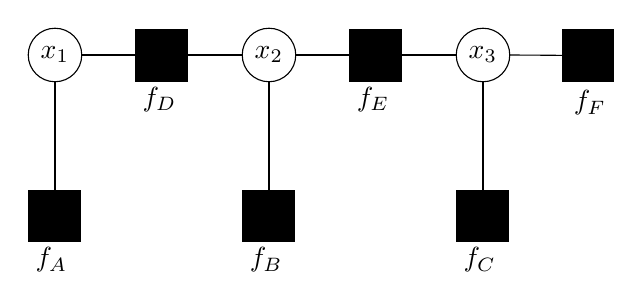
\begin{tikzpicture}[x=0.75pt,y=0.75pt,yscale=-1,xscale=1]
%uncomment if require: \path (0,288); %set diagram left start at 0, and has height of 288

%Shape: Square [id:dp542094098374186] 
\draw  [fill={rgb, 255:red, 0; green, 0; blue, 0 }  ,fill opacity=1 ] (86.34,228.71) -- (110.92,228.71) -- (110.92,253.29) -- (86.34,253.29) -- cycle ;
%Shape: Rectangle [id:dp9431678202688636] 
\draw  [fill={rgb, 255:red, 0; green, 0; blue, 0 }  ,fill opacity=1 ] (189.45,228.71) -- (214.03,228.71) -- (214.03,253.29) -- (189.45,253.29) -- cycle ;
%Shape: Rectangle [id:dp5515594438313509] 
\draw  [fill={rgb, 255:red, 0; green, 0; blue, 0 }  ,fill opacity=1 ] (292.57,228.71) -- (317.14,228.71) -- (317.14,253.29) -- (292.57,253.29) -- cycle ;
%Shape: Rectangle [id:dp19402149967725735] 
\draw  [fill={rgb, 255:red, 0; green, 0; blue, 0 }  ,fill opacity=1 ] (137.9,151.38) -- (162.47,151.38) -- (162.47,175.96) -- (137.9,175.96) -- cycle ;
%Shape: Rectangle [id:dp9723919948872586] 
\draw  [fill={rgb, 255:red, 0; green, 0; blue, 0 }  ,fill opacity=1 ] (241.01,151.38) -- (265.59,151.38) -- (265.59,175.96) -- (241.01,175.96) -- cycle ;
%Shape: Circle [id:dp9001944284946917] 
\draw   (86,163.41) .. controls (86,156.29) and (91.77,150.52) .. (98.89,150.52) .. controls (106.01,150.52) and (111.78,156.29) .. (111.78,163.41) .. controls (111.78,170.53) and (106.01,176.3) .. (98.89,176.3) .. controls (91.77,176.3) and (86,170.53) .. (86,163.41) -- cycle ;
%Shape: Ellipse [id:dp029985916423680425] 
\draw   (189.11,163.41) .. controls (189.11,156.29) and (194.88,150.52) .. (202,150.52) .. controls (209.12,150.52) and (214.89,156.29) .. (214.89,163.41) .. controls (214.89,170.53) and (209.12,176.3) .. (202,176.3) .. controls (194.88,176.3) and (189.11,170.53) .. (189.11,163.41) -- cycle ;
%Shape: Ellipse [id:dp8505763078012687] 
\draw   (292.22,163.41) .. controls (292.22,156.29) and (297.99,150.52) .. (305.11,150.52) .. controls (312.23,150.52) and (318,156.29) .. (318,163.41) .. controls (318,170.53) and (312.23,176.3) .. (305.11,176.3) .. controls (297.99,176.3) and (292.22,170.53) .. (292.22,163.41) -- cycle ;
%Straight Lines [id:da5591298719832298] 
\draw    (202,176.3) -- (202,236.1) ;
%Straight Lines [id:da8657801799701208] 
\draw    (305.11,176.3) -- (305.11,236.1) ;
%Straight Lines [id:da7323179142438296] 
\draw    (98.89,176.3) -- (98.89,236.1) ;
%Straight Lines [id:da2650402956705291] 
\draw    (141.85,163.41) -- (111.78,163.41) ;
%Straight Lines [id:da6929917679064295] 
\draw    (189.11,163.41) -- (159.04,163.41) ;
%Straight Lines [id:da7044874759875848] 
\draw    (244.96,163.41) -- (214.89,163.41) ;
%Straight Lines [id:da30371490539779855] 
\draw    (292.22,163.41) -- (262.15,163.41) ;
%Shape: Rectangle [id:dp26239558807935515] 
\draw  [fill={rgb, 255:red, 0; green, 0; blue, 0 }  ,fill opacity=1 ] (343.59,151.38) -- (368.16,151.38) -- (368.16,175.96) -- (343.59,175.96) -- cycle ;
%Straight Lines [id:da46629291479421253] 
\draw    (355.87,163.67) -- (318,163.41) ;


% Text Node
\draw (90.75,157.95) node [anchor=north west][inner sep=0.75pt]    {$x_{1}$};
% Text Node
\draw (193.86,157.95) node [anchor=north west][inner sep=0.75pt]    {$x_{2}$};
% Text Node
\draw (296.97,157.95) node [anchor=north west][inner sep=0.75pt]    {$x_{3}$};
% Text Node
\draw (88.3,255) node [anchor=north west][inner sep=0.75pt]    {$f_{A}$};
% Text Node
\draw (191.48,255) node [anchor=north west][inner sep=0.75pt]    {$f_{B}$};
% Text Node
\draw (294.53,255) node [anchor=north west][inner sep=0.75pt]    {$f_{C}$};
% Text Node
\draw (243.04,177.67) node [anchor=north west][inner sep=0.75pt]    {$f_{E}$};
% Text Node
\draw (139.79,177.67) node [anchor=north west][inner sep=0.75pt]    {$f_{D}$};
% Text Node
\draw (347.59,179.36) node [anchor=north west][inner sep=0.75pt]    {$f_{F}$};


\end{tikzpicture}


    \caption[Example factor graph]{An example of a factor graph}
\end{figure}

The above factor graph represents the following factorisation:

\begin{equation}
    p(X_1, X_2, X_3) = f_A(X_1)f_B(X_2)f_C(X_3)f_D(X_1, X_2)f_E(X_2, X_3)f_F(X_3)
    \label{eqn:factors}
\end{equation}

Assuming that each variable takes discrete values, suppose we wanted to find the probability that $X_1 = z$ for some value of $z$ using the above factor graph. Then we would need to find:

\begin{equation}
    p(X_1 = z, X_2, X_3) = \underset{i=X_2}{\sum} \underset{j=X_3}{\sum} p(X_1 = z, X_2 = i, X_3 =j)
    \label{eqn:bp_derivation_1}
\end{equation}

And by \ref{eqn:factors} we get:

\begin{equation}
    p(X_1 = z, X_2, X_3) = \underset{i=X_2}{\sum} \underset{j=X_3}{\sum} f_A(z)f_B(i)f_C(j)f_D(z, i)f_E(z, j)f_F(j)
\end{equation}


which can be rearranged to form:

\begin{equation}
    p(X_1 = z, X_2, X_3) = f_A(z) \underset{i=X_2}{\sum} \left(f_D(z, i)f_B(i) \left(\underset{j=X_3}{\sum} f_E(z, j)f_C(j)f_F(j) \right)\right)
    \label{eqn:x1}
\end{equation}

Similarly, if we wanted to find the probability that $X_2 = z$ for some z we would need to find:

\begin{equation}
    p(X_1, X_2 = z, X_3) = f_b(z) \left(\underset{i=X_1}{\sum} f_D(i, z) f_A(i)\right) \left(\underset{j=X_3}{\sum} f_E(z, j) f_C(j) f_F(j)\right)
    \label{eqn:x2}
\end{equation}

Noticing how the sum over $X_3$ in both \ref{eqn:x1} and \ref{eqn:x2} is the same, we may want to ``cache'' the result when dealing with large factor graphs, to improve performance. To do this we can associate calculations with nodes in the factor graph. We call these associations ``messages''.

The general form of a message from variable $i$ to factor $j$ is the product of the messages from all other neighbouring factors \cite{GaussianBP}. Formally:

\begin{equation}
    m_{x_i \rightarrow f_j} = \underset{s \in N(i) \backslash j }{\prod} m_{f_s \rightarrow x_i}
    \label{eqn:v_f}
\end{equation}

The general form of a message from factor $j$ to variable $i$ is the product of the messages from all other neighbouring variables and the factor applied to all other variables except $i$ \cite{GaussianBP}. Put formally:

\begin{equation}
    m_{f_j \rightarrow x_i} = \left(\underset{X_j \backslash x_i}{\sum} f_j(X_j)\right) \left(\underset{k \in N(j) \backslash i}{\prod} m_{x_k \rightarrow f_j}\right)
    \label{eqn:f_v}
\end{equation}

Finally, the marginal value (belief) of a variable is simply the product of all incoming messages to it \cite{GaussianBP}.

\begin{equation}
    p(x_i) = \underset{s \in N(i)}{\prod} m_{f_s \rightarrow x_i}
    \label{eqn:bp_belief}
\end{equation}

\subsection{Belief Propagation}
The above equations are used by the Belief Propagation algorithm, an iterative message-passing algorithm used to calculate the marginal value for each variable in a factor graph \cite{GaussianBP}. Each iteration of Belief Propagation has 3 phases:

\begin{enumerate}
    \item Variables send messages to each of their neighbouring factors \ref{eqn:v_f}.
    \item Factors send messages to each of their neighbouring variables \ref{eqn:f_v}.
    \item Each variable updates its ``belief'' (its estimated marginal value) \ref{eqn:bp_belief}.
\end{enumerate}

The original Belief Propagation algorithm was designed to be used in tree-like graphs, i.e. graphs without loops \cite{GaussianBP}. However, empirical evidence has shown that ``Loopy-BP'' can still converge to provide useful results in a variety of problem domains \cite{GaussianBP}. % TODO replace citations with better ones 

\subsection{Gaussian Belief Propagation}
A special case of the Belief Propagation algorithm is Gaussian Belief Propagation, which applies to problems where all variables follow a Gaussian distribution, and all factors are Gaussian functions of their inputs.

Under Gaussian Belief Propagation, each message can be interpreted as a Gaussian and so must contain sufficient information to produce one. A naive way of achieving this is to include a mean vector and a covariance matrix in each message. However, this approach is computationally expensive as it requires a full matrix multiplication whenever messages are multiplied which is an order $O(n^3)$ operation. An alternative approach is to use the \textit{canonical form} of the multivariate Gaussian distribution.

The canonical form uses an \textit{information vector} ($\eta$) and a \textit{precision matrix} ($\Lambda$) defined as follows:

\begin{align*}
    \eta = \Sigma^{-1} \mu && \Lambda = \Sigma^{-1}
\end{align*}

where $\Sigma$ is the covariance matrix and $\mu$ is the mean vector. Now multiplying messages is made more efficient as it only requires the addition of both messages' $\eta$ and $\Lambda$ values, making it an order $O(n^2)$ operation in the worst case. A further performance improvement can be made by recognising that the precision matrix is sparse \cite{GaussianBP}.

\unsure{Should I add equations for gbp?}

\subsection{Lie Theory}
Lie theory is a subset of group theory focussed on studying \textit{Lie groups}. Lie theory is a vast and abstract field, from which we only need to borrow a few concepts. The first is that positions and rotations can be represented as Lie groups, for example, the group $SO2$ represents a rotation in 2D space and the $SE3$ group represents a rigid motion in 3D space. The second core concept is the \textit{tangent space} which allows small deviations to be applied to the Lie group uniformly regardless of the value it operates on. This concludes our whirlwind tour of Lie theory, we invite the reader to read \cite{MicroLieTheory} for a more detailed tutorial.

% QUESTION: Do I need this at all?
% A group is a set of elements $G$ combined with a composition operation $\circ$, such that the following properties hold:
% \begin{enumerate}
%     \item Composing 2 elements of G results in another element of G
%     \item There exists an identity element $\epsilon$ so that composing any element with $\epsilon$ or $\epsilon$ with any element results in the same element
%     \item Composing an element with its inverse results in $\epsilon$
%     \item Composition is associative
% \end{enumerate}

% A Lie group is a group combined with a smooth manifold

\subsection{Putting it all together}
Now that we have covered all of the prerequisites to understanding how the Robot Web operates, we shall now demonstrate how they can be assembled into the Robot Web.

Every robot in the Robot Web needs to estimate its current location at all times, this is called localisation. One simple localisation method is to use odometry, which uses internal sensors to measure its displacement from its previous location. Since no sensor is perfect, this introduces a small amount of noise, which can be accurately modelled using a Gaussian distribution. The Robot Web simulates odometry using a factor graph, each known position of the robot maps to a pose variable, and the variables of each pair of successive positions are connected by an odometry factor. On every timestep, the robot performs an iteration of Gaussian Belief Propagation to estimate its current position.

The Robot Web further improves the accuracy of robots' locations by allowing robots to measure each other using external sensors. When a robot senses another, it creates a factor in its factor graph between its and the other's latest pose variables. When each robot wants to send a message to another, it publishes the message to its \textbf{Robot Web Page}, which the other robot will eventually read and use to update its location estimate.

\begin{figure}[!h]
    \centering
    

\tikzset{every picture/.style={line width=0.75pt}} %set default line width to 0.75pt        

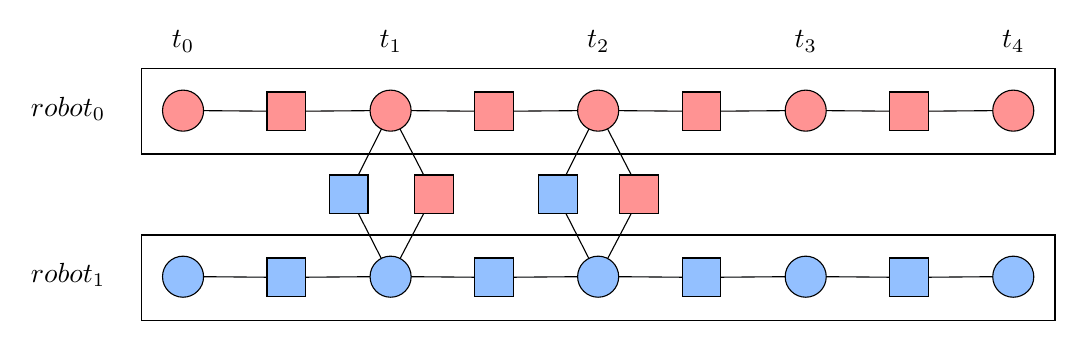
\begin{tikzpicture}[x=0.75pt,y=0.75pt,yscale=-1,xscale=1]
%uncomment if require: \path (0,288); %set diagram left start at 0, and has height of 288

%Straight Lines [id:da47036734988196627] 
\draw    (299.67,170.04) -- (319.89,209.71) ;
%Straight Lines [id:da6881382794521629] 
\draw    (319.89,129.71) -- (299.67,170.04) ;
%Straight Lines [id:da3959117741800886] 
\draw    (319.89,129.71) -- (340.67,170.04) ;
%Straight Lines [id:da6282284807536171] 
\draw    (340.67,170.04) -- (319.89,209.71) ;
%Straight Lines [id:da5198960712037324] 
\draw    (199.67,170.04) -- (219.89,209.71) ;
%Straight Lines [id:da8902598554725618] 
\draw    (219.89,129.71) -- (199.67,170.04) ;
%Straight Lines [id:da2738660568678817] 
\draw    (219.89,129.71) -- (240.67,170.04) ;
%Straight Lines [id:da06728554169051759] 
\draw    (240.67,170.04) -- (219.89,209.71) ;
%Straight Lines [id:da34036055728120096] 
\draw [fill={rgb, 255:red, 255; green, 147; blue, 147 }  ,fill opacity=1 ]   (329.78,129.71) -- (369.67,130.04) ;
%Straight Lines [id:da8072322510197338] 
\draw [fill={rgb, 255:red, 255; green, 147; blue, 147 }  ,fill opacity=1 ]   (369.67,130.04) -- (410,129.71) ;
%Straight Lines [id:da405451058550087] 
\draw [fill={rgb, 255:red, 255; green, 147; blue, 147 }  ,fill opacity=1 ]   (429.78,129.71) -- (469.67,130.04) ;
%Straight Lines [id:da7616794610228106] 
\draw [fill={rgb, 255:red, 255; green, 147; blue, 147 }  ,fill opacity=1 ]   (469.67,130.04) -- (510,129.71) ;
%Straight Lines [id:da6814419083610201] 
\draw [fill={rgb, 255:red, 255; green, 147; blue, 147 }  ,fill opacity=1 ]   (229.78,129.71) -- (269.67,130.04) ;
%Straight Lines [id:da7724102331322766] 
\draw [fill={rgb, 255:red, 255; green, 147; blue, 147 }  ,fill opacity=1 ]   (269.67,130.04) -- (310,129.71) ;
%Straight Lines [id:da5821529621200299] 
\draw [fill={rgb, 255:red, 255; green, 147; blue, 147 }  ,fill opacity=1 ]   (169.67,130.04) -- (210,129.71) ;
%Straight Lines [id:da0542087989667579] 
\draw [fill={rgb, 255:red, 255; green, 147; blue, 147 }  ,fill opacity=1 ]   (129.78,129.71) -- (169.67,130.04) ;
%Shape: Square [id:dp4499442483222458] 
\draw  [fill={rgb, 255:red, 255; green, 147; blue, 147 }  ,fill opacity=1 ] (160.34,120.71) -- (179,120.71) -- (179,139.37) -- (160.34,139.37) -- cycle ;
%Shape: Circle [id:dp2600881142320077] 
\draw  [fill={rgb, 255:red, 255; green, 147; blue, 147 }  ,fill opacity=1 ] (110,129.71) .. controls (110,124.25) and (114.43,119.82) .. (119.89,119.82) .. controls (125.35,119.82) and (129.78,124.25) .. (129.78,129.71) .. controls (129.78,135.17) and (125.35,139.6) .. (119.89,139.6) .. controls (114.43,139.6) and (110,135.17) .. (110,129.71) -- cycle ;
%Shape: Rectangle [id:dp7305091073359651] 
\draw   (100,109.6) -- (540,109.6) -- (540,150.6) -- (100,150.6) -- cycle ;
%Shape: Square [id:dp49665350033925293] 
\draw  [fill={rgb, 255:red, 255; green, 147; blue, 147 }  ,fill opacity=1 ] (260.34,120.71) -- (279,120.71) -- (279,139.37) -- (260.34,139.37) -- cycle ;
%Shape: Circle [id:dp8551402235390253] 
\draw  [fill={rgb, 255:red, 255; green, 147; blue, 147 }  ,fill opacity=1 ] (210,129.71) .. controls (210,124.25) and (214.43,119.82) .. (219.89,119.82) .. controls (225.35,119.82) and (229.78,124.25) .. (229.78,129.71) .. controls (229.78,135.17) and (225.35,139.6) .. (219.89,139.6) .. controls (214.43,139.6) and (210,135.17) .. (210,129.71) -- cycle ;
%Shape: Square [id:dp6259568957324568] 
\draw  [fill={rgb, 255:red, 255; green, 147; blue, 147 }  ,fill opacity=1 ] (360.34,120.71) -- (379,120.71) -- (379,139.37) -- (360.34,139.37) -- cycle ;
%Shape: Circle [id:dp7516686593765485] 
\draw  [fill={rgb, 255:red, 255; green, 147; blue, 147 }  ,fill opacity=1 ] (310,129.71) .. controls (310,124.25) and (314.43,119.82) .. (319.89,119.82) .. controls (325.35,119.82) and (329.78,124.25) .. (329.78,129.71) .. controls (329.78,135.17) and (325.35,139.6) .. (319.89,139.6) .. controls (314.43,139.6) and (310,135.17) .. (310,129.71) -- cycle ;
%Shape: Square [id:dp4907257696393781] 
\draw  [fill={rgb, 255:red, 255; green, 147; blue, 147 }  ,fill opacity=1 ] (460.34,120.71) -- (479,120.71) -- (479,139.37) -- (460.34,139.37) -- cycle ;
%Shape: Circle [id:dp40511868636697557] 
\draw  [fill={rgb, 255:red, 255; green, 147; blue, 147 }  ,fill opacity=1 ] (410,129.71) .. controls (410,124.25) and (414.43,119.82) .. (419.89,119.82) .. controls (425.35,119.82) and (429.78,124.25) .. (429.78,129.71) .. controls (429.78,135.17) and (425.35,139.6) .. (419.89,139.6) .. controls (414.43,139.6) and (410,135.17) .. (410,129.71) -- cycle ;
%Shape: Circle [id:dp7561415264055935] 
\draw  [fill={rgb, 255:red, 255; green, 147; blue, 147 }  ,fill opacity=1 ] (510,129.71) .. controls (510,124.25) and (514.43,119.82) .. (519.89,119.82) .. controls (525.35,119.82) and (529.78,124.25) .. (529.78,129.71) .. controls (529.78,135.17) and (525.35,139.6) .. (519.89,139.6) .. controls (514.43,139.6) and (510,135.17) .. (510,129.71) -- cycle ;
%Straight Lines [id:da6629990224165134] 
\draw [fill={rgb, 255:red, 147; green, 192; blue, 255 }  ,fill opacity=1 ]   (329.78,209.71) -- (369.67,210.04) ;
%Straight Lines [id:da6819695700249584] 
\draw [fill={rgb, 255:red, 147; green, 192; blue, 255 }  ,fill opacity=1 ]   (369.67,210.04) -- (410,209.71) ;
%Straight Lines [id:da7961157322315353] 
\draw [fill={rgb, 255:red, 147; green, 192; blue, 255 }  ,fill opacity=1 ]   (429.78,209.71) -- (469.67,210.04) ;
%Straight Lines [id:da7688161886956275] 
\draw [fill={rgb, 255:red, 147; green, 192; blue, 255 }  ,fill opacity=1 ]   (469.67,210.04) -- (510,209.71) ;
%Straight Lines [id:da8267819717164204] 
\draw [fill={rgb, 255:red, 147; green, 192; blue, 255 }  ,fill opacity=1 ]   (229.78,209.71) -- (269.67,210.04) ;
%Straight Lines [id:da5116263132351999] 
\draw [fill={rgb, 255:red, 147; green, 192; blue, 255 }  ,fill opacity=1 ]   (269.67,210.04) -- (310,209.71) ;
%Straight Lines [id:da7065942165163066] 
\draw [fill={rgb, 255:red, 147; green, 192; blue, 255 }  ,fill opacity=1 ]   (169.67,210.04) -- (210,209.71) ;
%Straight Lines [id:da6801634542744135] 
\draw [fill={rgb, 255:red, 147; green, 192; blue, 255 }  ,fill opacity=1 ]   (129.78,209.71) -- (169.67,210.04) ;
%Shape: Square [id:dp5838901472847389] 
\draw  [fill={rgb, 255:red, 147; green, 192; blue, 255 }  ,fill opacity=1 ] (160.34,200.71) -- (179,200.71) -- (179,219.37) -- (160.34,219.37) -- cycle ;
%Shape: Circle [id:dp8237018481465868] 
\draw  [fill={rgb, 255:red, 147; green, 192; blue, 255 }  ,fill opacity=1 ] (110,209.71) .. controls (110,204.25) and (114.43,199.82) .. (119.89,199.82) .. controls (125.35,199.82) and (129.78,204.25) .. (129.78,209.71) .. controls (129.78,215.17) and (125.35,219.6) .. (119.89,219.6) .. controls (114.43,219.6) and (110,215.17) .. (110,209.71) -- cycle ;
%Shape: Rectangle [id:dp1468154649235054] 
\draw   (100,189.6) -- (540,189.6) -- (540,230.6) -- (100,230.6) -- cycle ;
%Shape: Square [id:dp21555253881823844] 
\draw  [fill={rgb, 255:red, 147; green, 192; blue, 255 }  ,fill opacity=1 ] (260.34,200.71) -- (279,200.71) -- (279,219.37) -- (260.34,219.37) -- cycle ;
%Shape: Circle [id:dp8554188945699046] 
\draw  [fill={rgb, 255:red, 147; green, 192; blue, 255 }  ,fill opacity=1 ] (210,209.71) .. controls (210,204.25) and (214.43,199.82) .. (219.89,199.82) .. controls (225.35,199.82) and (229.78,204.25) .. (229.78,209.71) .. controls (229.78,215.17) and (225.35,219.6) .. (219.89,219.6) .. controls (214.43,219.6) and (210,215.17) .. (210,209.71) -- cycle ;
%Shape: Square [id:dp5941665721073983] 
\draw  [fill={rgb, 255:red, 147; green, 192; blue, 255 }  ,fill opacity=1 ] (360.34,200.71) -- (379,200.71) -- (379,219.37) -- (360.34,219.37) -- cycle ;
%Shape: Circle [id:dp5825532487467875] 
\draw  [fill={rgb, 255:red, 147; green, 192; blue, 255 }  ,fill opacity=1 ] (310,209.71) .. controls (310,204.25) and (314.43,199.82) .. (319.89,199.82) .. controls (325.35,199.82) and (329.78,204.25) .. (329.78,209.71) .. controls (329.78,215.17) and (325.35,219.6) .. (319.89,219.6) .. controls (314.43,219.6) and (310,215.17) .. (310,209.71) -- cycle ;
%Shape: Square [id:dp7753119223119171] 
\draw  [fill={rgb, 255:red, 147; green, 192; blue, 255 }  ,fill opacity=1 ] (460.34,200.71) -- (479,200.71) -- (479,219.37) -- (460.34,219.37) -- cycle ;
%Shape: Circle [id:dp5771019164898812] 
\draw  [fill={rgb, 255:red, 147; green, 192; blue, 255 }  ,fill opacity=1 ] (410,209.71) .. controls (410,204.25) and (414.43,199.82) .. (419.89,199.82) .. controls (425.35,199.82) and (429.78,204.25) .. (429.78,209.71) .. controls (429.78,215.17) and (425.35,219.6) .. (419.89,219.6) .. controls (414.43,219.6) and (410,215.17) .. (410,209.71) -- cycle ;
%Shape: Circle [id:dp21210412845989923] 
\draw  [fill={rgb, 255:red, 147; green, 192; blue, 255 }  ,fill opacity=1 ] (510,209.71) .. controls (510,204.25) and (514.43,199.82) .. (519.89,199.82) .. controls (525.35,199.82) and (529.78,204.25) .. (529.78,209.71) .. controls (529.78,215.17) and (525.35,219.6) .. (519.89,219.6) .. controls (514.43,219.6) and (510,215.17) .. (510,209.71) -- cycle ;
%Shape: Square [id:dp7557733799934572] 
\draw  [fill={rgb, 255:red, 147; green, 192; blue, 255 }  ,fill opacity=1 ] (190.34,160.71) -- (209,160.71) -- (209,179.37) -- (190.34,179.37) -- cycle ;
%Shape: Square [id:dp8894509337156504] 
\draw  [fill={rgb, 255:red, 255; green, 147; blue, 147 }  ,fill opacity=1 ] (231.34,160.71) -- (250,160.71) -- (250,179.37) -- (231.34,179.37) -- cycle ;
%Shape: Square [id:dp6301411170449531] 
\draw  [fill={rgb, 255:red, 255; green, 147; blue, 147 }  ,fill opacity=1 ] (330.34,160.71) -- (349,160.71) -- (349,179.37) -- (330.34,179.37) -- cycle ;
%Shape: Square [id:dp8001210630138842] 
\draw  [fill={rgb, 255:red, 147; green, 192; blue, 255 }  ,fill opacity=1 ] (291.34,160.71) -- (310,160.71) -- (310,179.37) -- (291.34,179.37) -- cycle ;

% Text Node
\draw (113.3,90) node [anchor=north west][inner sep=0.75pt]    {$t_{0}$};
% Text Node
\draw (213.3,90) node [anchor=north west][inner sep=0.75pt]    {$t_{1}$};
% Text Node
\draw (313.3,90) node [anchor=north west][inner sep=0.75pt]    {$t_{2}$};
% Text Node
\draw (413.3,90) node [anchor=north west][inner sep=0.75pt]    {$t_{3}$};
% Text Node
\draw (513.3,90) node [anchor=north west][inner sep=0.75pt]    {$t_{4}$};
% Text Node
\draw (45.3,122) node [anchor=north west][inner sep=0.75pt]    {$robot_{0}$};
% Text Node
\draw (45.3,202) node [anchor=north west][inner sep=0.75pt]    {$robot_{1}$};


\end{tikzpicture}

    \caption[Robot Web factor graph]{An example of a factor graph in the Robot Web. Each robot's variables are connected by odometry factors. At times $t_1$ and $t_2$, both robots sense each other, and so exchange measurements by creating inter-robot-measurement factors on the graph.}
\end{figure}

%TODO - the real reason for lie groups is to nicely apply gaussians
The Robot Web represents the locations and sensor measurements of all robots using general Lie groups, rather than any specific group. This has the consequence that any type of sensor or robot can be a part of the Robot Web. For example, a drone moving in 3D space can interact with a car moving on a plane.

\subsection{Evaluation}
The Robot Web has been shown to improve the accuracy of robot localisation, and most importantly the inter-robot measurements have been shown to provide further improvements over schemes where robots would only measure landmarks. % TODO citation needed?

Furthermore, the Robot Web has proven to be robust to a large number of faulty inter-robot sensors reporting random measurements, with this robustness lasting until 70-80\% of inter-robot sensors reported corrupted measurements.

\begin{figure}[!h]
    \centering
    \includegraphics[page=1,width=.60\textwidth]{diagrams/sensor_noise.pdf}
    \caption[RobotWeb's robustness to garbage measurements]{A graph showing that the RobotWeb is robust to up to 70-80\% of ``garbage'' measurements, where faulty sensors report random measurements. ATE refers to the average Absolute Trajectory Error measured over 50 runs in an environment with 50 robots and 10 beacons running for 100 timesteps. Taken from \cite[Figure~5]{Robotweb}}
\end{figure}

Although the Robot Web is robust to many inter-robot sensors reporting random measurements, it is not robust to a bad actor which may instead report incorrect measurements designed to worsen the localisation of other members of the Robot Web. Possible attacks include but are not limited to:

\begin{enumerate}
    \item Sending messages with extremely high confidences, to lull others into a false sense of security.
    \item Sending these messages whilst assuming the identity of another robot.
    \item Sending these messages from many nonexistent robots, also known as a Sybil attack.
\end{enumerate}

\section{Security Issues}
In this section, we will discuss several general security issues that can arise in robot networks. We will focus on issues that affect the accuracy of a robot's internal model of the world. This excludes attacks which may result in an attacker gaining control over a robot, yet includes attacks performed by hijacked robots.

\subsection{Denial of Service} % Can go into more detail if necessary.
A denial of service attack seeks to deny service. In a robot network such as the Robot Web, this would prevent one or more robots from being able to access messages sent by their peers and essentially cut them off from the network.

The simplest way for an attacker to perform a DoS attack is to use a signal jammer, which can be constructed using off-the-shelf equipment \cite{SignalJamming}. This would continuously transmit signals within the range of frequencies allowed by the communication medium, both interfering with and irrecoverably corrupting any messages sent. More sophisticated attackers may craft harder-to-detect jammer attacks by mimicking legitimate messages or only transmitting when it senses communication \cite{SignalJamming}. In addition to these, there exist a whole host of jamming attacks (and defences) targetting specific communication protocols.

Another form of a DoS attack would be to disconnect specific robots from the network, using the network protocol's existing defences. For example, by convincing others that the target is a bad actor, triggering their defences to remove the target from the network. % Kinda like a de-authentication attack, but not really since we're not sending explicit de-authentication frames to do this.

\subsection{Identity-Based Attacks}
% One class of attacks that could wreak havoc on robot networks are identity-based attacks; here a nonzero number of bad actors, claim false identities, which may or may not correspond to other robots in the network. The former is known as a spoofing attack, whilst the latter constitutes a Sybil attack.

Identity-based attacks can wreak havoc on robot networks. Using the model defined by Douceur \cite{SybilAttack}, we can describe a robot network as one consisting of $E$ entities (robots) each claiming at least one identity $i$ from the set of all identities $I$. When the network is under an identity-based attack, at least one of the following two properties will hold: % TODO maybe add the faulty/correct distinction
\begin{enumerate}
    \item Two entities, $e1, e2$ will present the same identity $i$
    \item The number of identities in $I$ will exceed the number of entities in $E$.
\end{enumerate}
If only the former holds, then the network is under a spoofing attack, whereas if only the latter holds, then the network is under a Sybil attack. Note: there is no guarantee that only one of these will hold at a time, and so we must be prepared to defend against both simultaneously.

\subsubsection{Spoofing Attacks}
Devices exchange information by sending packets or frames of data. For our purposes, we can ignore the differences between packets and frames, and use the terms interchangeably. Packets are used to encapsulate the data sent with relevant metadata, such as the source and destination IDs of the packet. This metadata is the main target of spoofing attacks.

In a spoofing attack, the attacker first finds the identity of a legitimate device, for example by first intercepting packets and then extracting the source ID from them. After this point, the attacker sends misleading packets impersonating the target. 

This can have several benefits for the attacker. Firstly, they could covertly inject misinformation into the network by impersonating an already trusted robot. Secondly, they could trigger defences in the network to flag target for misinformation and remove it.

\subsubsection{Sybil Attacks}
In a Sybil attack, the attacker will create many fake identities to gain undue influence on the network. In a robot network, this would allow them to indirectly influence the actions of victim robots. For example, one could lead two self-driving cars to conclude that their best course of action is to crash, by claiming many false identities would be hit if they were not to.

Douceur \cite{SybilAttack} proves Sybil attacks are always possible in distributed systems where there is no central arbiter of truth. They present and prove four lemmas about identities in large-scale distributed systems. The first two lemmas are concerned with entities which directly validate the identities presented to them, whilst the second two lemmas involve entities which rely upon other, potentially untrustworthy, identities for validation. The lemmas are as follows:

 %TODO lemma-ise

\begin{enumerate}
    \item If an attacker has $\rho$ times as many resources as the weakest entity, then they can successfully present up to $\lfloor\rho\rfloor$ distinct identities.
    \item If an entity doesn't validate all identities simultaneously, then an attacker can present an unbounded number of distinct identities.
    \item If an entity trusts $q$ other identities to validate an identity, then at least $f$ attackers are required to perform the attack, where $f >= q$ or the resources commanded by the attackers exceed $q + f$ times the weakest entity's resources.
    \item If all $c$ non-attackers don't coordinate when they validate identities, and an entity again trusts $q$ other identities for validation, then even a weak attacker can present $\lfloor\frac{c}{q}\rfloor$ identities.
\end{enumerate}

We plan to solve this problem by treating the physical world as a central arbiter of truth, albeit with some degree of error, due to imperfections in sensors.

\subsection{Physical Attacks}
Finally, since this thesis focuses on the security of robot networks, we will discuss the possibility of physical attacks on the system, and our limited ability to protect against them. We define a physical attack as any attempt to compromise the ability of a robot to perform its task. This includes colliding with the robot but also includes more subtle tactics, such as obscuring the robot's sensors. Physical attacks could also be used similarly to Sybil attacks, where several attackers would surround a robot and feed it misinformation. 

In this thesis, we will not attempt to protect against attacks where several robots would physically collide, since this would require heavy hardware modifications to existing robots. Instead, we will focus on occlusion attacks and physical Sybil attacks, at the very least allowing a robot to detect them.\\
% \chapter{Related Work}
\noindent\makebox[\linewidth]{\rule{\textwidth}{1pt}}


Several different techniques have been explored in preventing the types of identity-based attacks discussed in this chapter. In the \nth{2} half of this chapter, we will examine and evaluate these. We broadly group these approaches into 2 main groups; the first uses the physical characteristics of signal propagation to bind an identity to an entity, whilst the second exploits the fact that no entity can perform an unlimited amount of computation.

\section{Wifi Fingerprinting}
% In this section, we will review two Wifi fingerprinting-based approaches to binding identities to entities. 

There are many ways for devices to communicate wirelessly, many of which use radiowaves. Wifi is the name of a family of networking protocols that allow for this, it derives from the IEEE 802.11 standard. In order to use Wifi, a device must have at least one wireless antenna which can transmit and receive within the bands specified in the IEEE 802.11 standard; usually 2.4GHz and 5GHz.

When a device sends a packet using Wifi, it transmits a radio signal for a given number of nanoseconds from its antenna. This signal will attenuate as it travels further and further through space. After a certain distance, also known as the communicating range of the antenna, the signal will fade into background noise. The signal leaves the antenna in all directions simultaneously, as a radio wave. Eventually, a small part of this wave will reach the receiver's antenna and the packet will be decoded out of it.

Other parts of the wave will either diffract around corners, reflect off some large objects, or scatter off many small objects \cite{SignalProp}. Consequently, this means that a receiver may receive a packet from several different directions simultaneously, that is that it could encounter different parts of the same wave from different directions at the same time. This phenomenon is known as multipath scattering. %TODO Add diagram? 

Multipath scattering has two interesting properties; it is practically impossible to predict, ahead of time, the distribution of signals around a receiver and it is unlikely that two receivers will observe the same signal propagation with sufficient multipath scattering\citationneeded. These properties allow for devices to ``fingerprint'' every packet they receive, such that two different transmitters cannot have the same fingerprint unless they are simultaneously located at the same place. 

However, implementing multipath scattering-based algorithms have some technical constraints; namely that the receiving antenna must be able to measure the signal in each direction, and that a sufficient amount of multipath scattering must occur. Usually, these algorithms struggle in outdoor environments, where the environment may not provide objects for multipath scattering to occur\citationneeded.

The following papers discuss methods to circumvent these constraints, focussing on securing robot networks from spoofing and Sybil attacks. 

\subsection{Guaranteeing spoof-resilient multi-robot networks}
Gil et al, \cite{GuaranteeingSpoofResilience} provides an interesting approach to some of the aforementioned problems, most notably the problem of requiring expensive hardware to allow the receiving antenna to measure the signal in each direction. They do this by inventing an algorithm that allows them to build a ``virtual spoofer sensor'' only using commercially available wifi hardware, which creates a ``spatial fingerprint'' from each transmission in the network. They use the output from this sensor to calculate a confidence metric $\alpha$ indicating their algorithm's confidence that a robot's identity is its entity. Finally, they characterise the theoretical performance of the ``virtual spoofer sensor'' and provide empirical evidence to support their claims by undertaking several experiments.

The authors build the ``virtual spoofer sensor'' by building upon \textit{Synthetic Aperture Radar} (SAR) techniques, which allow a single antenna to be used to simulate an antenna array. SAR involves moving the antenna to different locations and taking snapshots of the signals received. These snapshots are then combined using signal-processing techniques to emulate a multi-antenna array \cite{BAD_SAR}.\unsure{Diagram needed?}
%TODO: This isn't a great citation, go to the original paper
The ``spatial fingerprint'' calculated, is then compared to the fingerprints of other clients, and clients with identical fingerprints are assumed to be Sybil attackers.

The authors evaluate their algorithm in the context of the following problem statement. Given an environment with several ``clients'', each expecting service from mobile ``servers'', dynamically find the optimal layout for the servers such that each ``client'' is served. A subset of clients are assumed to be malicious and are carrying out Sybil attacks in order to influence the ``servers'' to move closer to them.

The authors perform four experiments to validate their hypotheses:
\begin{enumerate}
    \item They compare the performance of the ``virtual spoofer sensor'' in both an indoor and simulated outdoor environment, as expected, finding that multipath scattering is more effective in indoor settings, but also that adding a single reflector to the environment vastly improves performance.
    \item They compare the effect of a stationary, moving, and power-scaling Sybil attacker on the ability of the ``virtual spoofer sensor'' to correctly classify agents, resulting in no false negatives, but many false positives.
    \item They evaluate their system on the multi-agent coverage problem \cite{MultiAgentCoverage}, finding that it can provide near-optimal results even when there are 3$\times$ more spoofed agents.
    \item They apply their system to a drone delivery problem, where the ``server'' needs to visit each real ``client'' to deliver a package and again find that their system provides near-optimal results when there are 3$\times$ more spoofed agents.
\end{enumerate}

\unsure{I have suspicions about how they did the last 2 experiments, especially since the phantoms are nowhere near the actual attacker.}

\subsection{Lightweight Sybil-Resilient Multi-Robot Networks by Multipath Manipulation}
Huang et al. \cite{MultiPathManipulation} take a different approach to Gil et al. \cite{GuaranteeingSpoofResilience}; instead of relying upon the environment to provide multipath scattering, they actively cause it by using backscatter tags. This offers two main advantages over Gil et al.: \begin{enumerate*}
    \item the environment has a lesser effect on the performance of the Sybil attack detector and
    \item the robots' antennae no longer need to move when capturing a fingerprint.
\end{enumerate*}
Using the captured signal information, the robots again compute a fingerprint per transmission, normalise it to mitigate the effects of any power scaling attacks, and finally compare the normalised fingerprint to those of all others, treating any identities with sufficiently similar fingerprints as Sybil attackers.

Backscatter tags scatter signals that they encounter by rapidly absorbing and reflecting them. Backscatter tags also simplify the fingerprinting process, since robots are no longer required to perform small movements for SAR, nor must the software engage in expensive linear algebra to construct a multi-antenna array. 

A key property of backscatter tags is that they operate passively and don't require a power supply. This reduces the cost of implementing this scheme as tags can be simply and inexpensively attached to robots. Another useful property is that the backscattering of the final signal is highly correlated with the positions of the tags, transmitting and receiving antennae, meaning that if two identities have very similar backscattering patterns, they are likely to originate from the same entity.

When a robot receives a signal, it receives a raw signal, which is first smoothed out with a moving average filter, to create the backscattered signal. Then it decodes a message out of the backscattered signal, and uses it, with signal processing techniques to deduce how much each tag contributed to the backscattering, and when each tag was ``activated''. Then the robot does more filtering to remove any backscattering from the environment, the resulting signal will be used to construct a signature for the transmission.

The authors then evaluate their implementation in both an indoor office environment and an outdoor rooftop environment. They find that their method is virtually indifferent to the surrounding environment, as they measure an average true positive rate of 97.6\% and an average false positive rate of 5.1\%.

\subsection{Conclusions}

Although both sets of authors extensively test their system, they make some problematic assumptions, which may be exploited by attackers. 

\begin{enumerate}
    \item They do not account for Sybil attacks using multiple antennae, which could transmit the same message at the same time, but with variable power levels. Each antenna would create a different multipath scatter, and if the relative powers between them were varied, then they could theoretically construct many false fingerprints.
    \item They also do not account for collaboration between different attackers, which would function similarly to the previous vulnerability, where geographically distributed attackers could simultaneously send the same message, with different power scales, creating another set of false fingerprints. This method could produce a larger range of false identities but may encounter synchronisation problems between attackers.
    \item Attackers could leverage methods similar to Huang et al. and physically augment their antennae to manipulate their multipath scattering, for example, one could create moveable barriers to prevent some scattering from occurring.
    \item Both sets of authors assume that any noise from the environment will not be malicious; Gil et al. assume that it will follow a Gaussian distribution, whilst Huang et al. assume that standard signal processing techniques would be sufficient to filter it out. Both of these assumptions fail to account for the possibility that coordinated attackers emit noise above background levels, but not so high that it would seriously interfere with transmissions. This would disrupt every transmission's signature and would prevent any pair of transmissions from looking alike.
\end{enumerate}


% \todo{Add diagram for 3}

\section{Proof of Work}
Proof of Work is underpinned by the insight that no entity in a network can perform unlimited computation. This leads to defences reliant on the idea that generating identities should be computationally expensive, to prevent any entity from being able to create an unbounded number of them. A PoW identity generation scheme would express an identity as the solution to some puzzle, and thus the identity can be validated by checking if it is a valid solution to the puzzle. This imposes two constraints: \begin{enumerate*}
    \item the puzzle must be hard to solve and
    \item the solution to a puzzle must be easy to verify
\end{enumerate*}, which means that, formally, the puzzle belongs to the \textit{NP-Complete} class of problems.

A problem with this strategy is that it requires wasting computational resources, which may be in short supply for the embedded systems used in robotics. Furthermore, it requires that normal robots constantly pay a steep price for their security even without the presence of attackers.

Gupta et al. \cite{PoW} design an iterative algorithm (\textbf{GMCom}) that solves the \nthM{2} problem, where if attackers spend $T$ resources, whilst $J$ new non-attacking identities are presented, then each non-attacker only needs to spend $O(\sqrt[2]{TJ} + J)$ resources. They refer to this property as the \textit{assymetry} of the algorithm, as attackers must spend many more resources than non-attackers.

GMCom organises identities into a group, where a subset of them form a committee. When a new identity tries to join the group, it must first solve a puzzle set by the committee. Occasionally, the committee will seek to purge all attackers from the group, by issuing a \textit{purge puzzle}, which must be solved by all identities before a new committee is formed, otherwise the identity will be purged from the group. This limits the wasted computation that good entities must perform since they only need to solve a single puzzle when entering a group, and occasionally thereafter, whilst an attacker would need to solve puzzles for each identity it claims, and would need to solve them repeatedly to avoid being purged.

However, this approach is not without its limitations. The authors assume that attackers will always only be able to command a fraction, $\alpha$, of the total resources of the system, however, the heterogeneous nature of robots means that this may not always be guaranteed. For example, in a drone delivery system, each drone would likely only possess a small amount of computational power, but an attacker may attack the system using their desktop computer.

% GMCom organises identities into a group, where a subset of them form a committee. When a new identity tries to join the group, it must first solve a current epoch's puzzle, set by the committee, and broadcast its solution. Once a certain number of identities has joined or left the group, the committee starts the next epoch with a new puzzle and new committee. 
% \section{Attacks on sensor networks}
% \section{Reputation based systems}

\chapter{An Investigation into the Security of RobotWeb}
The goal of this chapter is to understand how attackers will affect the functioning of the RobotWeb. First, we will posture about the aims of attackers, and how they would pursue them. Then we will dedicate the remainder of the chapter to answering the question of how successful they can be; first theoretically then empirically.

\section{The behaviour of an ideal attacker}
The RobotWeb allows robots to improve their localisations; these are likely to be used for navigational or control purposes. If a robot believes that it is too far left, its navigation/control system will instruct it to move right. This link between localisation and action is the prize sought after by attackers. If an attacker wishes for a robot to move right, it must simply convince it that it has moved too far left.

In addition to compromising others' localisations, an attacker will wish to keep its localisation uncompromised. This would mean that it would ignore any messages from robots that it has attacked, lest it inadvertently misinforms itself. However, this will come at a cost to the attacker, as it has fewer good sources of information about its localisation. If an attacker attacks all robots around it, it would effectively cut itself out of the RobotWeb, which leads us to believe that attackers would seek to perform targeted attacks. Here the attackers would either only attack a small number of robots, or attack robots at key times. Motivated attackers, seeking to attack all robots, may instead use a private version of the RobotWeb, where their attacks don't affect them.

Attackers will also wish to prevent their attacks from being easily identified, as those can be easily defended against. If their attacks are defended against, the overall effectiveness of an attacker is greatly diminished. Thus it stands to reason that attackers would aim to blend into the crowd, where their messages are indistinguishable from good messages. This means that an attacker is unlikely to try to convince robots that they are 100s of kilometers away, instead opting for more subtle differences.

Finally, when multiple attackers are present in an environment, it would be best for them to collaborate rather than compete. Competing attackers are likely to interfere with each others' attacks and thus reduce their overall efficacy. For this reason, we will ignore situations where this occurs.


\section{A simplified system}
Any theoretical investigation of the RobotWeb would require the investigator to analyse its backbone, the factor graph. However, the investigator would soon find themselves ensnared by complexity; caught in an intricate web of variable and factor nodes; messages constantly scurrying between them. Worse yet, the web would constantly be spun and unspun as robots moved closer and further from each other. In the face of this complexity, it becomes clear that simplification is needed.

To start, we choose to limit our investigation to a single variable, chosen arbitrarily, in the factor graph. Fortunately, the properties of Belief Propagation allow us to reason about this variable without loss of generality. Equation \ref{eqn:bp_belief} shows that the belief of a given variable is solely dependent on its connected factors. 

\begin{figure}[!h]
	\centering
	

\tikzset{every picture/.style={line width=0.75pt}} %set default line width to 0.75pt        

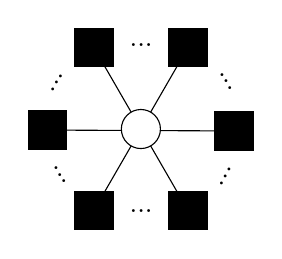
\begin{tikzpicture}[x=0.75pt,y=0.75pt,yscale=-1,xscale=1]
%uncomment if require: \path (0,288); %set diagram left start at 0, and has height of 288

%Shape: Square [id:dp5011100430912303] 
\draw  [fill={rgb, 255:red, 0; green, 0; blue, 0 }  ,fill opacity=1 ] (221.44,121.44) -- (240,121.44) -- (240,140) -- (221.44,140) -- cycle ;
%Shape: Square [id:dp1834276888413744] 
\draw  [fill={rgb, 255:red, 0; green, 0; blue, 0 }  ,fill opacity=1 ] (199.12,159.78) -- (217.68,159.78) -- (217.68,178.34) -- (199.12,178.34) -- cycle ;
%Shape: Square [id:dp4346063530366504] 
\draw  [fill={rgb, 255:red, 0; green, 0; blue, 0 }  ,fill opacity=1 ] (199.12,81.22) -- (217.68,81.22) -- (217.68,99.78) -- (199.12,99.78) -- cycle ;
%Straight Lines [id:da04926983509243965] 
\draw    (230.72,130.72) -- (140.72,130.28) ;
%Straight Lines [id:da6042872004378272] 
\draw    (208.4,169.06) -- (163.04,90.5) ;
%Straight Lines [id:da23454228445560488] 
\draw    (163.04,169.06) -- (208.4,90.5) ;
%Shape: Circle [id:dp7060474924289566] 
\draw  [fill={rgb, 255:red, 255; green, 255; blue, 255 }  ,fill opacity=1 ] (176.31,129.78) .. controls (176.31,124.59) and (180.53,120.37) .. (185.72,120.37) .. controls (190.91,120.37) and (195.13,124.59) .. (195.13,129.78) .. controls (195.13,134.97) and (190.91,139.19) .. (185.72,139.19) .. controls (180.53,139.19) and (176.31,134.97) .. (176.31,129.78) -- cycle ;
%Shape: Square [id:dp12209236616988428] 
\draw  [fill={rgb, 255:red, 0; green, 0; blue, 0 }  ,fill opacity=1 ] (131.44,121) -- (150,121) -- (150,139.56) -- (131.44,139.56) -- cycle ;
%Shape: Square [id:dp4564996494162272] 
\draw  [fill={rgb, 255:red, 0; green, 0; blue, 0 }  ,fill opacity=1 ] (153.76,159.78) -- (172.32,159.78) -- (172.32,178.34) -- (153.76,178.34) -- cycle ;
%Shape: Square [id:dp4857190958072921] 
\draw  [fill={rgb, 255:red, 0; green, 0; blue, 0 }  ,fill opacity=1 ] (153.76,81.22) -- (172.32,81.22) -- (172.32,99.78) -- (153.76,99.78) -- cycle ;

% Text Node
\draw (225,100) node [anchor=north west][inner sep=0.75pt]  [rotate=-60] [align=left] {...};
% Text Node
\draw (221.25,157.5) node [anchor=north west][inner sep=0.75pt]  [rotate=60] [align=left] {...};
% Text Node
\draw (179,87.5) node [anchor=north west][inner sep=0.75pt]   [align=left] {...};
% Text Node
\draw (145,145) node [anchor=north west][inner sep=0.75pt]  [rotate=-60] [align=left] {...};
% Text Node
\draw (179,167.5) node [anchor=north west][inner sep=0.75pt]   [align=left] {...};
% Text Node
\draw (140,112.5) node [anchor=north west][inner sep=0.75pt]  [rotate=60] [align=left] {...};


\end{tikzpicture}

	\caption[Single Variable in a Factor Graph]{A single variable connected to a number of factors}
\end{figure}

One problem still remains with the above setup - a single variable can be connected to any number of factors. As a further simplification, we can group the factors together based on their shared characteristics, which include their origin (if they are internal to the robot or not), their type (what kind of sensor they represent) and their intentions (whether they will help or hinder the robot). For our purposes, we will split the set of factors $F$, into distinct sets $G$ and $B$ based on whether the factors are ``good'' or ``bad'' for the robot. Good factors aim to steer the variable towards the ground truth value, while bad factors aim to steer it away. Notice that the sets $G$ and $B$ form a cover of $F$, that is $F = G \cup B$.

We then take this a step further and replace each set of factors with a single ``representative factor''.
\begin{figure}[!h]
	\centering
	

\tikzset{every picture/.style={line width=0.75pt}} %set default line width to 0.75pt        

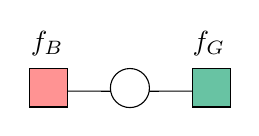
\begin{tikzpicture}[x=0.75pt,y=0.75pt,yscale=-1,xscale=1]
%uncomment if require: \path (0,171); %set diagram left start at 0, and has height of 171

%Straight Lines [id:da9426074160582016] 
\draw    (399.22,143.78) -- (359.94,143.66) ;
%Straight Lines [id:da643000004312603] 
\draw    (399.22,143.78) -- (438.5,143.66) ;
%Shape: Circle [id:dp3724334158586291] 
\draw  [fill={rgb, 255:red, 255; green, 255; blue, 255 }  ,fill opacity=1 ] (389.81,142.22) .. controls (389.81,137.03) and (394.02,132.81) .. (399.22,132.81) .. controls (404.41,132.81) and (408.62,137.03) .. (408.62,142.22) .. controls (408.62,147.41) and (404.41,151.63) .. (399.22,151.63) .. controls (394.02,151.63) and (389.81,147.41) .. (389.81,142.22) -- cycle ;
%Shape: Square [id:dp37804195853429245] 
\draw  [fill={rgb, 255:red, 255; green, 147; blue, 147 }  ,fill opacity=1 ] (350.66,132.81) -- (369.22,132.81) -- (369.22,151.37) -- (350.66,151.37) -- cycle ;
%Shape: Square [id:dp19659269496953535] 
\draw  [fill={rgb, 255:red, 104; green, 195; blue, 163 }  ,fill opacity=1 ] (429.22,132.81) -- (447.78,132.81) -- (447.78,151.37) -- (429.22,151.37) -- cycle ;

% Text Node
\draw (428.22,113.4) node [anchor=north west][inner sep=0.75pt]    {$f_{G}$};
% Text Node
\draw (350.22,113.4) node [anchor=north west][inner sep=0.75pt]    {$f_{B}$};


\end{tikzpicture}


	\caption[Representative factor graph around a single variable]{The above factor graph using ``representative factors''. $f_G$ and $f_B$ respectively represent the sets of good factors ($G$) and bad factors ($B$).}
\end{figure}

We calculate the messages from each of these representative factors as such:
\begin{eqnarray}
	m_{f_G \rightarrow x_i} = \underset{g \in G}{\prod} m_{f_g \rightarrow x_i}&
	m_{f_B \rightarrow x_i} = \underset{b \in B}{\prod} m_{f_b \rightarrow x_i}
\end{eqnarray}
Thus the belief of the variable becomes $p(x) = m_{f_G \rightarrow x} m_{f_B \rightarrow x}$, and since $G \cup B$ covers every factor connected to the variable, we can show that this replacement can be made without altering the variable's final result by equation \ref{eqn:bp_belief}.

\begin{equation}
	p(x_i) = \underset{s \in N(i)}{\prod} m_{f_s \rightarrow x_i}
	\tag{\ref{eqn:bp_belief}}
\end{equation}

For completeness, we now present the equations for contents of the messages $m_{f_G \rightarrow x_i}$ and $m_{f_B \rightarrow x_i}$. 
Each message has an information vector $\eta$ and a precision matrix $\Lambda$.
\begin{eqnarray}
	\eta_G = \underset{g \in G}{\sum} \eta_g&
	\Lambda_G = \underset{g \in G}{\sum} \Lambda_g \label{eqn:good_pull}\\
	\eta_B = \underset{b \in B}{\sum} \eta_b&
	\Lambda_B = \underset{b \in B}{\sum} \Lambda_b \label{eqn:bad_pull}
\end{eqnarray}

\section{Theoretical properties of the RobotWeb under attack}
\subsection{Measuring the strength of an attack}
From the above setup, we will now aim to quantify the strength of an attack. For mathematical convenience and ease of understanding, we will derive these equations in 1 dimension, and later present the n-dimensional forms.

To measure the strength of an attack we want to understand the impact of the bad factors on the variable's final belief. To do this we shall use the Kullback-Leibler (KL) divergence \citationneeded between the variable's belief when it is safe and when it is under attack.
The KL divergence is a measure of far the distribution Q is from the distribution P. The further the belief distribution under attack (BDA) is from the distribution suggested by the good factors, the stronger we say the attack is. Similarly, the closer the BDA is to the distribution suggested by the bad factors, the stronger the attack.

The KL divergence between 2 distributions of continuous random variables is:
\begin{equation}
	D_{KL}(P || Q) = \int_{-\infty}^{\infty} log\left( \frac{p(x)}{q(x)} \right) dx
\end{equation}

However a special case exists for Normal distributions, $N_1(\mu_1, \sigma_1^2)$ and $N_2(\mu_2, \sigma_2^2)$.
\begin{equation}
	D_{KL}(N_1 || N_2) = log\left(\frac{\sigma_2}{\sigma_1}\right) + \frac{\sigma_1^2 + (\mu_1 - \mu_2)^2}{2\sigma_2^2} - \frac{1}{2}
\end{equation}

In 1 dimension the messages sent from $f_G$ and $f_B$ are:
\begin{eqnarray}
	m_{f_G \rightarrow x_i} = (\eta_G, \Lambda_G) = (\frac{\mg}{\sgsq}, \frac{1}{\sgsq})\\
	m_{f_B \rightarrow x_i} = (\eta_B, \Lambda_B) = (\frac{\mb}{\sbsq}, \frac{1}{\sbsq}) \label{eqn:attacker_msg}
\end{eqnarray}

From \ref{eqn:bp_belief} we see that the BDA is equal to:
\begin{align}
	m_{f_G \rightarrow x} m_{f_B \rightarrow x} 
	&= (\eta_G + \eta_B, \Lambda_G + \Lambda_B)\\
	&= \left(\frac{\mg}{\sgsq} + \frac{\mb}{\sbsq}, \frac{1}{\sgsq} + \frac{1}{\sbsq}\right)\\
	&= \left(\frac{\mg\sbsq + \mb\sgsq}{\sgsq \sbsq}, \frac{\sbsq + \sgsq}{\sgsq \sbsq}\right)
\end{align}

The above distributions follow the following Normal distributions:
\begin{align}
	G &\sim N\left(\frac{\eta_G}{\Lambda_G}, \frac{1}{\Lambda_G}\right)\\
	B &\sim N\left(\frac{\eta_B}{\Lambda_B}, \frac{1}{\Lambda_B}\right)\\
	BDA &\sim N\left(\mu_{BDA}, \sigma_{BDA}^2\right)\\
	&\sim N\left(\frac{\eta_G + \eta_B}{\Lambda_G + \Lambda_B}, \frac{1}{\Lambda_G + \Lambda_B}\right)\\
	&\sim N\left(\frac{\mg\sbsq + \mb\sgsq}{\sgsq + \sbsq}, \frac{\sgsq \sbsq}{\sgsq + \sbsq}\right) \label{eqn:bda_distribution}
\end{align}

So now we take the KL divergence between the good factors' distribution $G$ and BDA. To make this easier to follow we derive each term in the sum separately.

First deriving the log term we get:
\begin{align}
	log\left(\frac{\sigma_{BDA}}{\sigma_{G}}\right)
	&= log\left(\sqrt[2]{\frac{\sigma_{BDA}^2}{\sigma_{G}^2}}\right)\\
	&= \frac{1}{2} log\left(\frac{\sigma_{BDA}^2}{\sigma_{G}^2}\right)\\
	&= \frac{1}{2} log\left(\frac{\sgsq \sbsq}{\sbsq + \sgsq} \times \frac{1}{\sgsq}\right)\\
	&= \frac{1}{2} log\left(\frac{\sbsq}{\sbsq + \sgsq}\right)
\end{align}

Next, we derive the fractional term:
\begin{align}
	\frac{\sigma_{G}^2 + (\mu_{G} - \mu_{BDA})^2}{2\sigma_{BDA}^2}
	&= \frac{
			\sgsq + \left(\mg - \frac{\mg\sbsq + \mb\sgsq}{\sbsq + \sgsq}\right)^2
		}{
			2 \frac{\sgsq \sbsq}{\sbsq + \sgsq}
		}\\
	&= \left(\sgsq + \left(\frac{\mg\sgsq + \mg\sbsq - \mg\sbsq - \mb\sgsq}{\sbsq + \sgsq}\right)^2\right) \times \frac{\sbsq + \sgsq}{2\sgsq\sbsq}\\
	&= \left(\sgsq + \left(\frac{\mg\sgsq - \mb\sgsq}{\sbsq + \sgsq}\right)^2\right) \times \frac{\sbsq + \sgsq}{2\sgsq\sbsq}\\
	&= \frac{\sgsq\left(\sgsq + \sbsq\right)^2 + \left(\mg\sgsq - \mb\sgsq\right)^2}{(\sbsq + \sgsq)^2} \times \frac{\sbsq + \sgsq}{2\sgsq\sbsq}\\
	&= \frac{\sgsq\left(\sgsq + \sbsq\right)^2 + \sigma_G^4\left(\mg - \mb\right)^2}{(\sbsq + \sgsq)^2} \times \frac{\sbsq + \sgsq}{2\sgsq\sbsq}\\
	&= \frac{\left(\sgsq + \sbsq\right)^2 + \sgsq\left(\mg - \mb\right)^2}{2\sbsq(\sbsq + \sgsq)}
\end{align}

Thus the KL divergence between $G$ and BDA is:
\begin{equation}
	\frac{1}{2} log\left(\frac{\sbsq}{\sbsq + \sgsq}\right) + \frac{\left(\sgsq + \sbsq\right)^2 + \sgsq\left(\mg - \mb\right)^2}{2\sbsq(\sbsq + \sgsq)} - \frac{1}{2}
\end{equation}

Similarly, the KL divergence between $B$ and BDA is:
\begin{equation}
	\frac{1}{2} log\left(\frac{\sgsq}{\sbsq + \sgsq}\right) + \frac{\left(\sgsq + \sbsq\right)^2 + \sbsq\left(\mg - \mb\right)^2}{2\sgsq(\sbsq + \sgsq)} - \frac{1}{2}
\end{equation}

From this, we notice a disturbing detail - the KL divergence is quadratically affected by the $\mb$. This suggests that the attacker's power is unbounded, so long as it chooses an appropriate $\sbsq$. This means that an attacker can suggest absurd localisations and have its victims believe them. For example, an attacker can convince its victims that they are on the opposite side of the planet!

\subsection{Crafting the perfect message}
From the results derived in the previous section, we know that, theoretically, an attacker will seek to increase its $\mb$ to $\infty$ and decrease its $\sbsq$ to 0. However, in a real-life scenario, it is unlikely that the attacker would fully exploit these powers, for two reasons.
\begin{enumerate}
	\item Robots are unlikely to believe \textit{incredibly} incorrect values - no sensible robot would believe that it has moved 500km away in the past 3 seconds.
	\item Robots don't have infinite numerical precision, so large values of $\Lambda_B$ ($\frac{1}{\sbsq}$) would cause overflow errors, which would prevent the attacker from controlling the robot's belief.
\end{enumerate}

Given these restrictions, attackers would set their values of $\mb$ to believable values, whilst choosing the largest value of $\sbsq$ possible. 
We will now suppose that the attacker wishes to move its victim's belief from $\mg$ to $\mt$.
As before, the attacker sends a message with the form described in equation \ref{eqn:attacker_msg}.

So from equation \ref{eqn:bda_distribution}, we see that:
\begin{equation}
	\mt = \frac{\mg\sbsq + \mb\sgsq}{\sgsq + \sbsq}
\end{equation}

Which can be rearranged into the form:
\begin{equation}
	\mb = \frac{\mt\left(\sgsq + \sbsq\right) - \mg\sbsq}{\sgsq}
\end{equation}

Which can be used to calculate the $\mb$ that an attacker would send given a minimum $\sbsq$. 
Thus the attacker would send the following message:
\begin{equation}
	\left(\frac{\mt\left(\sgsq + \sbsq\right) - \mg\sbsq}{\sgsq\sbsq}, \frac{1}{\sbsq}\right)
\end{equation}

\subsection{Scaling back up to n-dimensional space}
For completeness, we now present the KL divergence between the BDA and G distributions in k-dimensions.

The KL divergence between 2 k-variate Normal distributions, $N_1(\boldsymbol{\mu_1}, \Sigma_1)$ and $N_2(\boldsymbol{\mu_2}, \Sigma_2)$ is:
\begin{equation}
	KL\left[P || Q \right] = \frac{1}{2}\left[
		tr(\Sigma_2^{-1}\Sigma_1) + \left(\boldsymbol{\mu_2} - \boldsymbol{\mu_1}\right)^T \Sigma_2^{-1} \left(\boldsymbol{\mu_2} - \boldsymbol{\mu_1}\right) - k + log\left(\frac{det \; \Sigma_2}{det \; \Sigma_1}\right)
	\right]
\end{equation}

Using this with the messages sent from $f_G$ and $f_B$, we find that the KL divergence between G and BDA is:

\begin{gather}
	\frac{1}{2} \left[
		tr\left(\Lambda_B\Lambda_G^{-1}\right) +
		\left(\boldsymbol{\mu_{BDA}} - \boldsymbol{\mu_G}\right)^T \left(\Lambda_G + \Lambda_B\right) \left(\boldsymbol{\mu_{BDA}} - \boldsymbol{\mu_G}\right) + log\left(\frac{det \; \Lambda_G}{det \; \left(\Lambda_G + \Lambda_B\right)}\right)
	\right]\\
	\text{where}\nonumber\\
	\boldsymbol{\mu_{BDA}} = \left(\Lambda_G + \Lambda_B\right) \left(\eta_G + \eta_B\right)\nonumber
\end{gather}

\subsection{The Force-Based model of attacks}
From the above analysis, we believe that attacks can be reasoned about using a ``Force-Based Model''. Here we think of all messages sent to a variable as forces pulling the variable to particular localisations. Every good message will pull the variable towards the ground truth value, whilst every bad message will pull it towards an alternative localisation. The strength of a message's ``pull'' corresponds to the eigenvalues of its $\Lambda$ matrix, where the higher the eigenvalues, the stronger the pull is.

If two messages pull the robot towards the same localisation, then their forces will be additively combined, increasing their overall strength. However, if the messages pull the robot to diametrically opposed localisations, then their forces will cancel out. Once all forces have been resolved, the variable will move to the localisation suggested by the resultant force. The strength of the variable's conviction is determined by the strength of this resultant force.

\section{Hypotheses}
Now using the ``Force-Based Model'', we form 6 hypotheses about the behaviour of the entire RobotWeb under attack. Later, we will experimentally verify each of these hypotheses.

\subsection{There is Strength in Numbers} \label{hyp:strength_in_numbers}
As the number of good robots rises, the effectiveness of an attack will fall. We believe that this can be seen through the lens of the ``Force-Based Model'' where, as the number of good robots increases, so does the overall number of good messages, which in turn increases the overall force pulling the robots towards the truth. This will increase the resistance against any given attack, decreasing the strength of the resultant force.

However, it is unlikely that a large number of good robots will be able to nullify attacks, as the attacker will likely respond by increasing the strength of its messages. Since the good robots cannot freely increase $\Lambda$, they will once again conform to the attacker's wishes.

\subsection{Long Memories are Detrimental} \label{hyp:history} % History can be weaponised
One little discussed feature of the RobotWeb so far has been its time-windowed history. Instead of remembering every past position that that robot has had, it instead chooses to only remember the past $h$ positions. This improves the performance of robots in the RobotWeb, as they store fewer pose variables and thus perform fewer floating-point operations when updating beliefs. In the original paper, Murai et al. show that the impact of time-windowed history on the average performance of each robot is negligible.

%TODO: get original

\begin{figure}[!h]
    \centering
    \makebox[\textwidth]{\includegraphics[width=\textwidth]{diagrams/history.png}}
	\caption[The negligible effect of using time-windowed history]{Graphs showing a negligible decrease in performance between using a full history vector and only using the previous 5 pose variables. Taken from \cite[Figure~3]{Robotweb}}
\end{figure}


However, we believe that keeping the full position history not only harms the computational performance of a robot but also amplifies the strength of attacks. If an attacker can successfully attack a robot at time $t$, then the pose variable at $t$, $v_t$ will contain a $\mu$ close to the attacker's target $\mu$, and its $\Lambda$ will be high. Then in the next step, this corrupted $v_t$ will pull the robot towards the attacker's target instead of towards a ground truth. As the size of this history increases, so does the total pull it will have on the robot.

Note: During the early stages of an attack, we believe that longer histories will serve as a small counterbalance to the attacker, but as their strength is limited, they will be unable to significantly prevent an attack. Thus we believe that they are more harmful than helpful.

\subsection{Attacks are Contagious} \label{hyp:contagion} % A falling tide sinks all ships/Can't let the genie out of the bottle
Similarly to the previous hypothesis, we can assume that any other variable connected to $v_t$ will be attacked by it. Thus a victim of an attack will unintentionally attack all those it contacts, leading us to hypothesise that attacks have a degree of contagion. 

Attackers may not be able to prevent or limit contagion, as they would need to strongly pull unintentional victims back to a ground truth value. Since no robot has absolute certainty about the locations of any other, the attacker will pull them to values close to their ground truth. Yet, as there is no mechanism to decrease $\Lambda$, the attacker will still make the other robots overconfident about their locations, which may bias them in the long term.

\subsection{Young Robots are the most Vulnerable} \label{hyp:startup_vuln}
Robots which are have only recently joined the RobotWeb (and hence can be considered ``young'') are unlikely to have strong beliefs about their localisation. As they participate in the RobotWeb, the strength of their beliefs will increases. However, these initial weak beliefs will translate to a weaker pull towards the ground truth, and provide a weaker resistance to attackers.

We believe that this effect may be strongly linked to the robot's history size, as once the history size has been exhausted, the robot will only make marginal gains from experience.

\subsection{Bounds on $\mu$ can be slowly escaped} \label{hyp:mu_bound}
An intuitive defence against the attackers is setting an upper bound on how far a message can suggest the robot is from its current position belief. 
However, we believe that this approach is ineffective, and can be easily evaded by attackers. In this subsection, we will lay out how this defence would work and how it can be bypassed.

For the upper bound to be effective, it must occupy a ``Goldilocks zone'' - it cannot be too large or too small. If the upper bound is too large, it would present attackers with ample opportunities to control the robot's belief, especially since they aim to suggest somewhat plausible positions.
If the upper bound is too small, it would effectively prevent the robot from listening to any dissenting messages from other good robots.

Now suppose that at time $t$, the robot is at position $\mu_t$ and has an upper bound of $\epsilon$. It would then evaluate each incoming message and reject it if its proposed position $\mu'_t$ is a distance $\epsilon$ away from $\mu_t$. After filtering out all ``bad'' messages, the robot would use the remaining messages to determine $\mu_{t+1}$. 

Being aware of this scheme, an attacker would seek to incrementally attack the robot. It would start by proposing a position $\mu''_t$ that lies between $\mu_t$ and its target location $\mu'_t$, such that $\mu''_t$ is accepted by the robot. This would successfully shift the robot's position estimate $\mu_{t+1}$ to $\mu''_t$. In the next iteration, the robot would reject any proposals a distance of $\epsilon$ away from $\mu_{t+1} = \mu''_t$. Hence over several iterations, the robot's position estimate would slowly shift to $\mu'_t$, and thus the attacker would be able to escape the bound.
% \todo{Would a diagram be useful here?}

\subsection{Bounds on $\Lambda$ can be quickly escaped} \label{hyp:sybils}
As shown previously, the strength of an attack is highly dependent on its ability to propose arbitrary values of $\Lambda$. This leads to another intuitive defence strategy - robots set an upper bound on the $\Lambda$ values that they receive. We believe that this strategy is effective when there is only a single identity spreading misinformation, counterbalanced by many others sending reliable information. In this subsection, we will provide a justification for this belief as well as a strategy that an attacker could take to bypass the upper bound on $\Lambda$.

When sending a message, each robot decides the strength of the message's pull. Good robots limit their strength to the accuracy of their sensors, while attackers will set their strength to the fullest extent. This once again makes the case for the use of a reasonable upper bound on the strength of a message, similar to the one described above.

However, we argue that this upper bound is unenforceable in practice, for an attacker can simply ``split'' their message into several weaker parts. So far in our analysis, we have treated $\Lambda_B$ as if it were sent in a single message, however from equation \ref{eqn:bad_pull} we can see that it may also be the result of several bad robots sending messages. If the upper bound on an individual message's $\Lambda$ is $\lambda$, then an attacker could simply send several messages from several different identities to arrive at a strong $\Lambda_B$, in a Sybil Attack. Here the strengths of each Sybil's message will increase the overall strength of the attacking force, while each message's $\Lambda$ will fly under the bound.


\subsubsection{Aside: Attacks are uncorrelated} \label{hyp:uncorrelated_sybils}
Considering the ``Force-Based Model'' of variables, it stands to reason that in a Sybil Attack, the messages sent by individual identities will not be correlated with each other, as that would greatly simplify the detection and prevention of attacks. Instead, we believe that Sybil Attackers would send messages with wildly different $\mu$ values, that would resolve to the actual attack that the attacker intends.

Consequently, it becomes impossible to detect whether a message belongs to an attacker based on its contents.

\section{Experimental evidence}

Now, we will evaluate the above hypotheses in a simulated environment. Our goal is to show that the predicted phenomena can arise, rather than guaranteeing their emergence. The reasoning behind this is that an attack only needs to be successful in a single situation for it to be considered potent.

\subsection{Experimental setup}
We will use an adapted version of the simulator detailed in \cite[RobotWeb]{Robotweb} for our experiments. Each simulation will contain a single attacking robot and $n$ normal robots. Each robot will move along a predefined path, and aim to localise well to that path - this will be challenged by the attacker, which will attempt to trick them into localising to a path of its choosing.

Furthermore, each robot in the simulation will carry 2 sensors; one for odometry and one for measuring others. The odometry sensor will be used by a robot to estimate its current location using its previous location and its motion. The range-bearing sensor will be used to measure other robots - it will measure the distance between the 2 robots and the bearing of the other robot from this one. All robots' range-bearing sensors have a range limit; however, attackers will ignore this as they always know where they want their victims to be.

The simulation has several configurable parameters which we will vary in our experiments. We detail the most important ones below.

% TODO: make table good
% QUESTION: Should I explain how likely robots are to measure each other?
% TODO: Include startup delay
\renewcommand{\arraystretch}{1.35}
\begin{table}[ht!]
\centering
\begin{tabular}{|c|c|c|}
\hline
\textbf{Parameter}    & \textbf{Description}                                                                                                          & \textbf{Default values}                                                                                        \\ \hline
Dataset               & The physical path travelled by each robot.                                                                                    & See below                                                                                                      \\ \hline
Attacker Dataset      & \begin{tabular}[c]{@{}c@{}}The path attackers attempt to trick the robot \\ into localising onto\end{tabular}                 & See below                                                                                                      \\ \hline
History size & \begin{tabular}[c]{@{}c@{}}The number of past pose variables \\ used by each robot.\end{tabular} & 1                                                                                                             \\ \hline
N iterations per step & \begin{tabular}[c]{@{}c@{}}The number of GBP iterations performed\\  every time the robot moves.\end{tabular}                 & 10                                                                                                             \\ \hline
SE2 Prior             & The accuracy of each robot's original position.                                                                               & \begin{tabular}[c]{@{}c@{}}$\sigma_x = 1e^{-8}$ m\\ $\sigma_y = 1e^{-8}$ m\end{tabular}                        \\ \hline
Between SE2           & The accuracy of each robot's odometry sensor.                                                                                 & \begin{tabular}[c]{@{}c@{}}$\sigma_x = 0.1$ m\\  $\sigma_y = 0.1$ m \\ $\sigma_\theta = 0.01$ rad\end{tabular} \\ \hline
Sensor range limit    & The furthest a range-bearing sensor can detect.                                                                               & 0.25 m                                                                                                         \\ \hline
Sensor noise model    & \begin{tabular}[c]{@{}c@{}}The noise associated with the \\ range and bearing measurements.\end{tabular}                      & \begin{tabular}[c]{@{}c@{}}$\sigma_r = 0.05$ m\\ $\sigma_\theta = 0.1$ rad\end{tabular}                        \\ \hline
Attacker confidence   & \begin{tabular}[c]{@{}c@{}}The confidence claimed by the attacker.\end{tabular}                      & \begin{tabular}[c]{@{}c@{}}$\sigma_x = 0.001$ m\\ $\sigma_y = 0.001$ m\end{tabular} \\ \hline
\end{tabular}
\end{table}

\subsubsection{Path design}
Since the RobotWeb currently hasn't been deployed, we are faced with a dearth of real-world paths for our experiments. This leaves us with the choice of either inventing a realistic path or using a simple, artificial path. For the following experiments, we have chosen to use simple paths as we aim to show that these phenomena can arise. Later we will test our defences on more realistic paths.

\begin{figure}[!h]
	\centering
	

\tikzset{every picture/.style={line width=0.75pt}} %set default line width to 0.75pt        

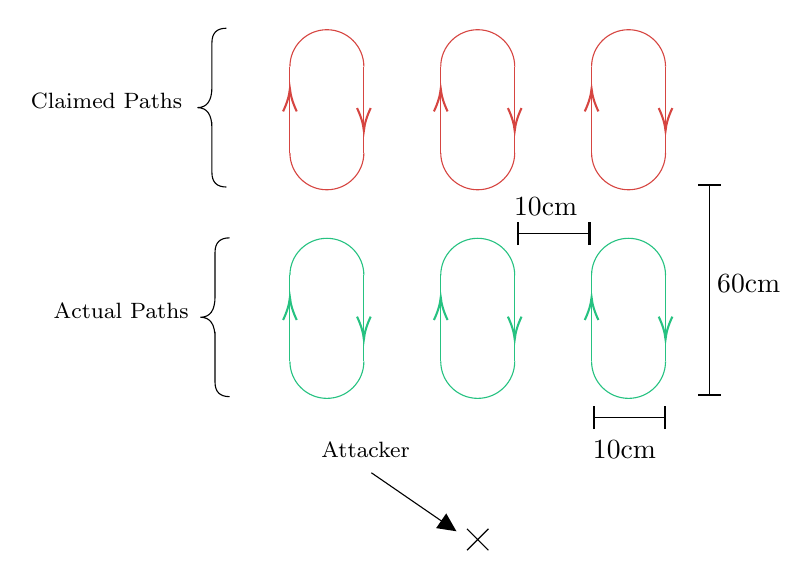
\begin{tikzpicture}[x=0.75pt,y=0.75pt,yscale=-1,xscale=1]
%uncomment if require: \path (0,300); %set diagram left start at 0, and has height of 300

%Shape: Arc [id:dp0857149156348076] 
\draw  [draw opacity=0] (129.08,53.57) .. controls (129.08,53.57) and (129.08,53.57) .. (129.08,53.57) .. controls (129.08,43.74) and (137.06,35.76) .. (146.9,35.76) .. controls (156.74,35.76) and (164.71,43.74) .. (164.71,53.57) -- (146.9,53.57) -- cycle ; \draw  [color={rgb, 255:red, 214; green, 69; blue, 65 }  ,draw opacity=1 ] (129.08,53.57) .. controls (129.08,53.57) and (129.08,53.57) .. (129.08,53.57) .. controls (129.08,43.74) and (137.06,35.76) .. (146.9,35.76) .. controls (156.74,35.76) and (164.71,43.74) .. (164.71,53.57) ;  
%Straight Lines [id:da5322421522198548] 
\draw [color={rgb, 255:red, 214; green, 69; blue, 65 }  ,draw opacity=1 ]   (129.08,53.57) -- (129.08,95.07) ;
%Shape: Arc [id:dp2308989347294783] 
\draw  [draw opacity=0] (164.71,95.07) .. controls (164.71,95.07) and (164.71,95.07) .. (164.71,95.07) .. controls (164.71,104.91) and (156.74,112.88) .. (146.9,112.88) .. controls (137.06,112.88) and (129.08,104.91) .. (129.08,95.07) -- (146.9,95.07) -- cycle ; \draw  [color={rgb, 255:red, 214; green, 69; blue, 65 }  ,draw opacity=1 ] (164.71,95.07) .. controls (164.71,95.07) and (164.71,95.07) .. (164.71,95.07) .. controls (164.71,104.91) and (156.74,112.88) .. (146.9,112.88) .. controls (137.06,112.88) and (129.08,104.91) .. (129.08,95.07) ;  
%Straight Lines [id:da5629844829721629] 
\draw [color={rgb, 255:red, 214; green, 69; blue, 65 }  ,draw opacity=1 ]   (164.71,53.57) -- (164.71,95.07) ;

%Straight Lines [id:da6879257912498304] 
\draw [color={rgb, 255:red, 214; green, 69; blue, 65 }  ,draw opacity=1 ]   (129.08,84.45) -- (129.08,66.19) ;
\draw [shift={(129.08,64.19)}, rotate = 90] [color={rgb, 255:red, 214; green, 69; blue, 65 }  ,draw opacity=1 ][line width=0.75]    (10.93,-3.29) .. controls (6.95,-1.4) and (3.31,-0.3) .. (0,0) .. controls (3.31,0.3) and (6.95,1.4) .. (10.93,3.29)   ;
%Straight Lines [id:da78952208923761] 
\draw [color={rgb, 255:red, 214; green, 69; blue, 65 }  ,draw opacity=1 ]   (164.71,82.45) -- (164.71,64.19) ;
\draw [shift={(164.71,84.45)}, rotate = 270] [color={rgb, 255:red, 214; green, 69; blue, 65 }  ,draw opacity=1 ][line width=0.75]    (10.93,-3.29) .. controls (6.95,-1.4) and (3.31,-0.3) .. (0,0) .. controls (3.31,0.3) and (6.95,1.4) .. (10.93,3.29)   ;

%Shape: Arc [id:dp943258450102171] 
\draw  [draw opacity=0] (201.75,53.57) .. controls (201.75,43.74) and (209.73,35.76) .. (219.57,35.76) .. controls (229.41,35.76) and (237.39,43.74) .. (237.39,53.57) -- (219.57,53.57) -- cycle ; \draw  [color={rgb, 255:red, 214; green, 69; blue, 65 }  ,draw opacity=1 ] (201.75,53.57) .. controls (201.75,43.74) and (209.73,35.76) .. (219.57,35.76) .. controls (229.41,35.76) and (237.39,43.74) .. (237.39,53.57) ;  
%Straight Lines [id:da7460858686327427] 
\draw [color={rgb, 255:red, 214; green, 69; blue, 65 }  ,draw opacity=1 ]   (201.75,53.57) -- (201.75,95.07) ;
%Shape: Arc [id:dp7505919410049695] 
\draw  [draw opacity=0] (237.39,95.07) .. controls (237.39,104.91) and (229.41,112.88) .. (219.57,112.88) .. controls (209.73,112.88) and (201.75,104.91) .. (201.75,95.07) -- (219.57,95.07) -- cycle ; \draw  [color={rgb, 255:red, 214; green, 69; blue, 65 }  ,draw opacity=1 ] (237.39,95.07) .. controls (237.39,104.91) and (229.41,112.88) .. (219.57,112.88) .. controls (209.73,112.88) and (201.75,104.91) .. (201.75,95.07) ;  
%Straight Lines [id:da5413783734225774] 
\draw [color={rgb, 255:red, 214; green, 69; blue, 65 }  ,draw opacity=1 ]   (237.39,53.57) -- (237.39,95.07) ;

%Straight Lines [id:da6345338713179298] 
\draw [color={rgb, 255:red, 214; green, 69; blue, 65 }  ,draw opacity=1 ]   (201.75,84.45) -- (201.75,66.19) ;
\draw [shift={(201.75,64.19)}, rotate = 90] [color={rgb, 255:red, 214; green, 69; blue, 65 }  ,draw opacity=1 ][line width=0.75]    (10.93,-3.29) .. controls (6.95,-1.4) and (3.31,-0.3) .. (0,0) .. controls (3.31,0.3) and (6.95,1.4) .. (10.93,3.29)   ;
%Straight Lines [id:da7349959112756272] 
\draw [color={rgb, 255:red, 214; green, 69; blue, 65 }  ,draw opacity=1 ]   (237.39,82.45) -- (237.39,64.19) ;
\draw [shift={(237.39,84.45)}, rotate = 270] [color={rgb, 255:red, 214; green, 69; blue, 65 }  ,draw opacity=1 ][line width=0.75]    (10.93,-3.29) .. controls (6.95,-1.4) and (3.31,-0.3) .. (0,0) .. controls (3.31,0.3) and (6.95,1.4) .. (10.93,3.29)   ;

%Shape: Arc [id:dp4454600887945992] 
\draw  [draw opacity=0] (274.42,53.57) .. controls (274.42,43.74) and (282.39,35.76) .. (292.23,35.76) .. controls (302.07,35.76) and (310.05,43.74) .. (310.05,53.57) -- (292.23,53.57) -- cycle ; \draw  [color={rgb, 255:red, 214; green, 69; blue, 65 }  ,draw opacity=1 ] (274.42,53.57) .. controls (274.42,43.74) and (282.39,35.76) .. (292.23,35.76) .. controls (302.07,35.76) and (310.05,43.74) .. (310.05,53.57) ;  
%Straight Lines [id:da3535450240320428] 
\draw [color={rgb, 255:red, 214; green, 69; blue, 65 }  ,draw opacity=1 ]   (274.42,53.57) -- (274.42,95.07) ;
%Shape: Arc [id:dp07519283691274281] 
\draw  [draw opacity=0] (310.05,95.07) .. controls (310.05,104.91) and (302.07,112.88) .. (292.23,112.88) .. controls (282.39,112.88) and (274.42,104.91) .. (274.42,95.07) -- (292.23,95.07) -- cycle ; \draw  [color={rgb, 255:red, 214; green, 69; blue, 65 }  ,draw opacity=1 ] (310.05,95.07) .. controls (310.05,104.91) and (302.07,112.88) .. (292.23,112.88) .. controls (282.39,112.88) and (274.42,104.91) .. (274.42,95.07) ;  
%Straight Lines [id:da4596754592263743] 
\draw [color={rgb, 255:red, 214; green, 69; blue, 65 }  ,draw opacity=1 ]   (310.05,53.57) -- (310.05,95.07) ;

%Straight Lines [id:da4148525058433936] 
\draw [color={rgb, 255:red, 214; green, 69; blue, 65 }  ,draw opacity=1 ]   (274.42,84.45) -- (274.42,66.19) ;
\draw [shift={(274.42,64.19)}, rotate = 90] [color={rgb, 255:red, 214; green, 69; blue, 65 }  ,draw opacity=1 ][line width=0.75]    (10.93,-3.29) .. controls (6.95,-1.4) and (3.31,-0.3) .. (0,0) .. controls (3.31,0.3) and (6.95,1.4) .. (10.93,3.29)   ;
%Straight Lines [id:da40569561359945716] 
\draw [color={rgb, 255:red, 214; green, 69; blue, 65 }  ,draw opacity=1 ]   (310.05,82.45) -- (310.05,64.19) ;
\draw [shift={(310.05,84.45)}, rotate = 270] [color={rgb, 255:red, 214; green, 69; blue, 65 }  ,draw opacity=1 ][line width=0.75]    (10.93,-3.29) .. controls (6.95,-1.4) and (3.31,-0.3) .. (0,0) .. controls (3.31,0.3) and (6.95,1.4) .. (10.93,3.29)   ;


%Shape: Arc [id:dp9600264214104561] 
\draw  [draw opacity=0] (129.08,154.07) .. controls (129.08,154.07) and (129.08,154.07) .. (129.08,154.07) .. controls (129.08,144.24) and (137.06,136.26) .. (146.9,136.26) .. controls (156.74,136.26) and (164.71,144.24) .. (164.71,154.07) -- (146.9,154.07) -- cycle ; \draw  [color={rgb, 255:red, 38; green, 194; blue, 129 }  ,draw opacity=1 ] (129.08,154.07) .. controls (129.08,154.07) and (129.08,154.07) .. (129.08,154.07) .. controls (129.08,144.24) and (137.06,136.26) .. (146.9,136.26) .. controls (156.74,136.26) and (164.71,144.24) .. (164.71,154.07) ;  
%Straight Lines [id:da06283910895753198] 
\draw [color={rgb, 255:red, 38; green, 194; blue, 129 }  ,draw opacity=1 ]   (129.08,154.07) -- (129.08,195.57) ;
%Shape: Arc [id:dp8022390792858354] 
\draw  [draw opacity=0] (164.71,195.57) .. controls (164.71,195.57) and (164.71,195.57) .. (164.71,195.57) .. controls (164.71,205.41) and (156.74,213.38) .. (146.9,213.38) .. controls (137.06,213.38) and (129.08,205.41) .. (129.08,195.57) -- (146.9,195.57) -- cycle ; \draw  [color={rgb, 255:red, 38; green, 194; blue, 129 }  ,draw opacity=1 ] (164.71,195.57) .. controls (164.71,195.57) and (164.71,195.57) .. (164.71,195.57) .. controls (164.71,205.41) and (156.74,213.38) .. (146.9,213.38) .. controls (137.06,213.38) and (129.08,205.41) .. (129.08,195.57) ;  
%Straight Lines [id:da5702202677205794] 
\draw [color={rgb, 255:red, 38; green, 194; blue, 129 }  ,draw opacity=1 ]   (164.71,154.07) -- (164.71,195.57) ;

%Straight Lines [id:da5596372875774243] 
\draw [color={rgb, 255:red, 38; green, 194; blue, 129 }  ,draw opacity=1 ]   (129.08,184.95) -- (129.08,166.69) ;
\draw [shift={(129.08,164.69)}, rotate = 90] [color={rgb, 255:red, 38; green, 194; blue, 129 }  ,draw opacity=1 ][line width=0.75]    (10.93,-3.29) .. controls (6.95,-1.4) and (3.31,-0.3) .. (0,0) .. controls (3.31,0.3) and (6.95,1.4) .. (10.93,3.29)   ;
%Straight Lines [id:da4662112490696484] 
\draw [color={rgb, 255:red, 38; green, 194; blue, 129 }  ,draw opacity=1 ]   (164.71,182.95) -- (164.71,164.69) ;
\draw [shift={(164.71,184.95)}, rotate = 270] [color={rgb, 255:red, 38; green, 194; blue, 129 }  ,draw opacity=1 ][line width=0.75]    (10.93,-3.29) .. controls (6.95,-1.4) and (3.31,-0.3) .. (0,0) .. controls (3.31,0.3) and (6.95,1.4) .. (10.93,3.29)   ;

%Shape: Arc [id:dp4562159985401648] 
\draw  [draw opacity=0] (201.75,154.07) .. controls (201.75,144.24) and (209.73,136.26) .. (219.57,136.26) .. controls (229.41,136.26) and (237.39,144.24) .. (237.39,154.07) -- (219.57,154.07) -- cycle ; \draw  [color={rgb, 255:red, 38; green, 194; blue, 129 }  ,draw opacity=1 ] (201.75,154.07) .. controls (201.75,144.24) and (209.73,136.26) .. (219.57,136.26) .. controls (229.41,136.26) and (237.39,144.24) .. (237.39,154.07) ;  
%Straight Lines [id:da19157667291963465] 
\draw [color={rgb, 255:red, 38; green, 194; blue, 129 }  ,draw opacity=1 ]   (201.75,154.07) -- (201.75,195.57) ;
%Shape: Arc [id:dp13013570223308513] 
\draw  [draw opacity=0] (237.39,195.57) .. controls (237.39,205.41) and (229.41,213.38) .. (219.57,213.38) .. controls (209.73,213.38) and (201.75,205.41) .. (201.75,195.57) -- (219.57,195.57) -- cycle ; \draw  [color={rgb, 255:red, 38; green, 194; blue, 129 }  ,draw opacity=1 ] (237.39,195.57) .. controls (237.39,205.41) and (229.41,213.38) .. (219.57,213.38) .. controls (209.73,213.38) and (201.75,205.41) .. (201.75,195.57) ;  
%Straight Lines [id:da19897438711687387] 
\draw [color={rgb, 255:red, 38; green, 194; blue, 129 }  ,draw opacity=1 ]   (237.39,154.07) -- (237.39,195.57) ;

%Straight Lines [id:da9802863492139731] 
\draw [color={rgb, 255:red, 38; green, 194; blue, 129 }  ,draw opacity=1 ]   (201.75,184.95) -- (201.75,166.69) ;
\draw [shift={(201.75,164.69)}, rotate = 90] [color={rgb, 255:red, 38; green, 194; blue, 129 }  ,draw opacity=1 ][line width=0.75]    (10.93,-3.29) .. controls (6.95,-1.4) and (3.31,-0.3) .. (0,0) .. controls (3.31,0.3) and (6.95,1.4) .. (10.93,3.29)   ;
%Straight Lines [id:da7197586821158186] 
\draw [color={rgb, 255:red, 38; green, 194; blue, 129 }  ,draw opacity=1 ]   (237.39,182.95) -- (237.39,164.69) ;
\draw [shift={(237.39,184.95)}, rotate = 270] [color={rgb, 255:red, 38; green, 194; blue, 129 }  ,draw opacity=1 ][line width=0.75]    (10.93,-3.29) .. controls (6.95,-1.4) and (3.31,-0.3) .. (0,0) .. controls (3.31,0.3) and (6.95,1.4) .. (10.93,3.29)   ;

%Shape: Arc [id:dp10249254547785802] 
\draw  [draw opacity=0] (274.42,154.07) .. controls (274.42,144.24) and (282.39,136.26) .. (292.23,136.26) .. controls (302.07,136.26) and (310.05,144.24) .. (310.05,154.07) -- (292.23,154.07) -- cycle ; \draw  [color={rgb, 255:red, 38; green, 194; blue, 129 }  ,draw opacity=1 ] (274.42,154.07) .. controls (274.42,144.24) and (282.39,136.26) .. (292.23,136.26) .. controls (302.07,136.26) and (310.05,144.24) .. (310.05,154.07) ;  
%Straight Lines [id:da6620574809946163] 
\draw [color={rgb, 255:red, 38; green, 194; blue, 129 }  ,draw opacity=1 ]   (274.42,154.07) -- (274.42,195.57) ;
%Shape: Arc [id:dp24299270541262064] 
\draw  [draw opacity=0] (310.05,195.57) .. controls (310.05,205.41) and (302.07,213.38) .. (292.23,213.38) .. controls (282.39,213.38) and (274.42,205.41) .. (274.42,195.57) -- (292.23,195.57) -- cycle ; \draw  [color={rgb, 255:red, 38; green, 194; blue, 129 }  ,draw opacity=1 ] (310.05,195.57) .. controls (310.05,205.41) and (302.07,213.38) .. (292.23,213.38) .. controls (282.39,213.38) and (274.42,205.41) .. (274.42,195.57) ;  
%Straight Lines [id:da3864874791920556] 
\draw [color={rgb, 255:red, 38; green, 194; blue, 129 }  ,draw opacity=1 ]   (310.05,154.07) -- (310.05,195.57) ;

%Straight Lines [id:da1738578603941392] 
\draw [color={rgb, 255:red, 38; green, 194; blue, 129 }  ,draw opacity=1 ]   (274.42,184.95) -- (274.42,166.69) ;
\draw [shift={(274.42,164.69)}, rotate = 90] [color={rgb, 255:red, 38; green, 194; blue, 129 }  ,draw opacity=1 ][line width=0.75]    (10.93,-3.29) .. controls (6.95,-1.4) and (3.31,-0.3) .. (0,0) .. controls (3.31,0.3) and (6.95,1.4) .. (10.93,3.29)   ;
%Straight Lines [id:da25617957855500695] 
\draw [color={rgb, 255:red, 38; green, 194; blue, 129 }  ,draw opacity=1 ]   (310.05,182.95) -- (310.05,164.69) ;
\draw [shift={(310.05,184.95)}, rotate = 270] [color={rgb, 255:red, 38; green, 194; blue, 129 }  ,draw opacity=1 ][line width=0.75]    (10.93,-3.29) .. controls (6.95,-1.4) and (3.31,-0.3) .. (0,0) .. controls (3.31,0.3) and (6.95,1.4) .. (10.93,3.29)   ;


%Straight Lines [id:da7311650809062149] 
\draw    (168.32,249.22) -- (206.85,275.72) ;
\draw [shift={(209.32,277.42)}, rotate = 214.52] [fill={rgb, 255:red, 0; green, 0; blue, 0 }  ][line width=0.08]  [draw opacity=0] (8.93,-4.29) -- (0,0) -- (8.93,4.29) -- cycle    ;
\draw   (214.4,276.22) -- (224.73,286.55)(224.73,276.22) -- (214.4,286.55) ;
%Shape: Brace [id:dp07511868864199678] 
\draw   (98.5,35.05) .. controls (93.83,35.05) and (91.5,37.38) .. (91.5,42.05) -- (91.5,63.3) .. controls (91.5,69.97) and (89.17,73.3) .. (84.5,73.3) .. controls (89.17,73.3) and (91.5,76.63) .. (91.5,83.3)(91.5,80.3) -- (91.5,104.55) .. controls (91.5,109.22) and (93.83,111.55) .. (98.5,111.55) ;
%Shape: Brace [id:dp4089807154309404] 
\draw   (100,136.05) .. controls (95.33,136.05) and (93,138.38) .. (93,143.05) -- (93,164.3) .. controls (93,170.97) and (90.67,174.3) .. (86,174.3) .. controls (90.67,174.3) and (93,177.63) .. (93,184.3)(93,181.3) -- (93,205.55) .. controls (93,210.22) and (95.33,212.55) .. (100,212.55) ;
%Straight Lines [id:da47101957924875837] 
\draw    (331.08,110.49) -- (331.08,211.68) ;
\draw [shift={(331.08,211.68)}, rotate = 270] [color={rgb, 255:red, 0; green, 0; blue, 0 }  ][line width=0.75]    (0,5.59) -- (0,-5.59)   ;
\draw [shift={(331.08,110.49)}, rotate = 270] [color={rgb, 255:red, 0; green, 0; blue, 0 }  ][line width=0.75]    (0,5.59) -- (0,-5.59)   ;
%Straight Lines [id:da6528183750796981] 
\draw    (310,222.55) -- (275.43,222.55) ;
\draw [shift={(275.43,222.55)}, rotate = 360] [color={rgb, 255:red, 0; green, 0; blue, 0 }  ][line width=0.75]    (0,5.59) -- (0,-5.59)   ;
\draw [shift={(310,222.55)}, rotate = 360] [color={rgb, 255:red, 0; green, 0; blue, 0 }  ][line width=0.75]    (0,5.59) -- (0,-5.59)   ;
%Straight Lines [id:da7816637873993619] 
\draw    (273.4,133.95) -- (238.83,133.95) ;
\draw [shift={(238.83,133.95)}, rotate = 360] [color={rgb, 255:red, 0; green, 0; blue, 0 }  ][line width=0.75]    (0,5.59) -- (0,-5.59)   ;
\draw [shift={(273.4,133.95)}, rotate = 360] [color={rgb, 255:red, 0; green, 0; blue, 0 }  ][line width=0.75]    (0,5.59) -- (0,-5.59)   ;

% Text Node
\draw (143.02,233.16) node [anchor=north west][inner sep=0.75pt]   [align=left] {{\footnotesize Attacker}};
% Text Node
\draw (14,166.16) node [anchor=north west][inner sep=0.75pt]   [align=left] {{\footnotesize Actual Paths}};
% Text Node
\draw (3,65.16) node [anchor=north west][inner sep=0.75pt]   [align=left] {{\footnotesize Claimed Paths}};
% Text Node
\draw (333.68,152.58) node [anchor=north west][inner sep=0.75pt]   [align=left] {60cm};
% Text Node
\draw (273.82,232.28) node [anchor=north west][inner sep=0.75pt]   [align=left] {10cm};
% Text Node
\draw (235.82,115.56) node [anchor=north west][inner sep=0.75pt]   [align=left] {10cm};


\end{tikzpicture}


	\caption[Paths used to evaluate attackers]{An example of the types of paths we use to test our hypotheses. In this example, there are 3 good robots and 1 attacking beacon. The attacker aims to shift the beliefs of its victims 60cm upwards.}
\end{figure}

We choose to use the above paths to test. The robots will move along the green path, whilst the attackers will try to convince them that they are instead moving along the red path. For these experiments, the attacker will take the form of a beacon placed at the bottom of the map.

%TODO: Sort out the measurement units

\subsection{Testing hypothesis 1}
The first hypothesis, \ref{hyp:strength_in_numbers}, predicts the existence of a ``strength in numbers'' effect, where the effectiveness of an attack is reduced as the number of good robots increases. We test this by varying the number of robots attacked and subsequently measuring the Average Trajectory Error (ATE) per robot. For a fair comparison, we extend the range of each robot's sensors to allow for every robot to sense every other robot. We repeat this experiment 10 times.
\begin{figure}[!h]
	\centering
	\subfigure[Including all loops]{
		\includegraphics[width=7cm]{graphs/n_bots_all_loops.pdf}
		\label{fig:strength-in-numbers-all}
	}
	\subfigure[Only including the final 3 loops]{
		\includegraphics[width=7cm]{graphs/n_bots_last_3_loops.pdf}
		\label{fig:strength-in-numbers-last-3}
	}
	\caption{The ``strength in numbers'' effect: as the number of robots increases, the effectiveness of an attack decreases. Note the outliers in \ref{fig:strength-in-numbers-all} occur as the weakened attacker is unable to instantly seize control of its victims.}
	\label{fig:strength-in-numbers}
\end{figure}

Looking at \ref{fig:strength-in-numbers}, we can see that a weak ``strength in numbers'' effect does exist, as the ATE decreases whilst the number of good robots increases. However, this effect was only observable after the attackers had been weakened, such that their $\sigma_X = \sigma_y = 1$m - which is a lower confidence level than all normal robots'.

Since this effect is only visible when attackers have been weakened, it is unlikely to present a significant hurdle to real-world attackers, unless they are vastly outnumbered. Therefore it is not a viable defence strategy.

\subsection{Testing hypothesis 2}
The second hypothesis, \ref{hyp:history}, suggests that robots keeping longer histories are more vulnerable to attacks. We test this using 2 robots; an attacker and its victim. We vary the victim's history size and measure its ATE. We again weaken the attacker's attacks by reducing its confidence such that $\sigma_x = \sigma_y = 10$ m. We repeat this experiment 10 times.

\begin{figure}[!h]
	\centering
	\subfigure[With attackers present]{
		\includegraphics[width=7cm]{graphs/history_size_all_loops.pdf}
		\label{fig:history-size-attackers}
	}
	\subfigure[Without any attackers present]{
		\includegraphics[width=7cm]{graphs/history_size_history_size_no_attackers_all_loops.pdf}
		\label{fig:history-size-no-attackers}
	}
	\caption{The effect of History Size on ATE: a longer history size is detrimental when attackers are present, yet provides little value otherwise.}
\end{figure}

Looking at \ref{fig:history-size-attackers} reveals that longer histories do harm robots' localisation, but only weakly. This is likely because the past poses are fully attacked by then, and so can't attack the robots further. However, \ref{fig:history-size-no-attackers} tells a different story about the value of longer histories. Here we see a negligible impact of longer history sizes on the ATE.

These results show that there is no advantage to be gained by using a longer history vector, which leads us to conclude that the history size should be kept at 1 to reduce the strength of attackers. This is likely to serve as an additional benefit as it reduces the overall computation required by members of the RobotWeb.

\subsection{Testing hypothesis 3}
The third hypothesis, \ref{hyp:contagion}, predicts that attacks will spread without the active involvement of the attacker, where the victims inadvertently will attack other robots. We test this using 12 robots; an attacker, its victim and 10 other robots. We devise a special configuration for this experiment where the attacker only communicates with its victim, and only adjacent robots can communicate with each other. This provides us with a daisy chain communication pattern, where the victim's attack must take several ``hops'' to reach the ends of the chain. We then measure the ATE of each robot over 10 runs. 

\begin{figure}[!h]
	\centering
	\subfigure[ATE vs Hops]{
		\includegraphics[width=7cm]{graphs/contagion_all_loops.pdf}
		\label{fig:contagion-boxplot}
	}
	\subfigure[ATE vs Time]{
		\includegraphics[width=7cm]{graphs/contagion_vs_time.pdf}
		\label{fig:contagion-vs-time}
	}
	\caption{The contagion effect: attacked robots slowly spread their attack out to their neighbours}
	\label{fig:contagion}
\end{figure}

Looking at \ref{fig:contagion-boxplot}, we can see that the fewer the number of hops from a robot to the victim, the higher its ATE will be, thus proving the existence of a contagion effect. However, we also see that the effect of the contagion decays, as the number of hops increases. This is likely because each victim does not \textit{try} to attack others, only doing so inadvertently, so the amount of influence it exerts on its neighbours is considerably lower than the influence the attacker exerts upon it. As a victim 1 hop away is less influenced, it too exerts less of an influence upon its neighbours. The overall effect of this is that the contagion is unlikely to spread rapidly and uncontrollably.

Looking at \ref{fig:contagion-vs-time}, we also see that the ATE of each affected robot increases linearly, which implies that given enough time, the contagion can overwhelm the RobotWeb.

This effect may somewhat deter real-world attackers from relying on any robots in the vicinity of their victims, lest they fall prey to their own attack, yet it is unlikely to act as an effective deterrent. A motivated attacker would instead find alternative means of localisation.

\subsection{Testing hypothesis 4}
The fourth hypothesis, \ref{hyp:startup_vuln}, posits that young robots which have recently joined the web will be the most vulnerable to attacks. We test using 2 robots; an attacker and its victim. We introduce a delay between when the victim starts and when it is attacked. We then measure the ATE of the victim across 10 runs. We also vary the victim's history size, as we believe that there is likely a link between the optimum startup delay of a robot and the size of its history. We once more weaken the attacker's attacks by reducing its confidence such that $\sigma_x = \sigma_y = 1$m.


\begin{figure}[!h]
	\centering
	\includegraphics[width=10cm]{graphs/startup_delay.pdf}
	\caption{The effect of a startup delay on the ATE, also investigating the effect of the history on this.}
	\label{fig:startup_delay}
\end{figure}

Note: This section is still a TODO because I realised that I made a mistake in the experiment.


\subsection{Testing hypothesis 5}
The fifth hypothesis, \ref{hyp:mu_bound}, predicts that attackers can overcome bounds on $\mu$, by performing incremental attacks. We test this using 2 robots; an attacker and its victim. For the victim, we introduce a $\mu$ bound defence of 0.05m, so that it only believes messages which are within a 0.05m radius from its current position estimate. For the attacker, we add an onramp composed of several segments, to transition the victim to the attacker's desired path. We vary the number of the onramp's segments and measure the victim's Average Trajectory Error (ATE) over 10 runs.


\begin{figure}[!h]
	\centering
	\subfigure[ATE vs Number of Onramp Segments]{
		\includegraphics[width=7cm]{graphs/mu_bound_last_3_loops_after_onramp.pdf}
		\label{fig:mu-bound-all}
	}
	\subfigure[ATE vs Time]{
		\includegraphics[width=7cm]{graphs/mu_bound_vs_time.pdf}
		\label{fig:mu-bound-vs-time}
	}
	\caption{Attackers escaping a 5cm $\mu$ bound: the 60cm difference between the actual and target path is bridged by n \textit{onramp segments} of equal lengths}
\end{figure}


Analysing the ATE against the number of segments, in \ref{fig:mu-bound-all}, we see that a cliff emerges, where once the segments are short enough, the ATE significantly increases, indicating a successful attack. Thus confirming that an attacker can easily overcome bounds on $\mu$.

Interestingly enough, we also see that the cliff starts when there are 12 segments. Here each segment would have a length of $\frac{0.6}{12} = 0.05$m, which is just outside the bound. This happens due to noise in the victim's localisation, which leads it to occasionally accept the attacker's messages. Every time the victim accepts one of these messages, it's pulled closer to the attacker's desired path, which in turn makes it more likely to accept the attacker's future messages.

Looking at the victim's ATE over time in \ref{fig:mu-bound-vs-time}, we see that the victim's ATE only increases once it is firmly on the onramp. In the case where there are 12 segments, we see that the victim only partially follows the target path, which is once again likely due to its noisy localisation. 

These results mean that although the $\mu$ bound defence can be evaded, it still hinders the attacker, which must both create an onramp and wait for its victim to traverse it.

\subsection{Testing hypothesis 6}
The sixth and final hypothesis, \ref{hyp:sybils}, asserts that an attacker can carry out an attack without manipulating its confidence level, instead the attacker would send many messages under many fake identities. We test this using 12 robots; an attacker and its 11 victims. We also prevent the attacker from altering the confidence level of any of the messages it sends. We vary the number of false identities that the attacker creates, and measure the average ATE across each victim. We repeat this experiment 10 times.

\begin{figure}[!ht]
	\centering
	\subfigure[caption]{
		\includegraphics[width=7cm]{graphs/sybils_all_loops.pdf}
		\label{fig:sybils}
	}
	\subfigure[caption]{
		\includegraphics[width=7cm]{graphs/sybils_vs_time.pdf}
		\label{fig:sybils-vs-time}
	}
	\caption{A Sybil attack on the RobotWeb: as the number of Sybils increases, so does the influence of the attacker upon the rest of the RobotWeb}
\end{figure}


From \ref{fig:sybils}, we see that the ATE quickly converges around 0.6m as the number of Sybils increases. We also see the spread of ATEs narrow. Both these facts confirm that the Sybil attack is highly effective against the RobotWeb. Notably, since the confidence level of messages sent from a Sybil is equal to that of those sent by normal robots, they blend in perfectly with normal messages. This means that a robot cannot determine the true state using messages alone. Furthermore, unlike the previous experiment, when we analyse the ATE over time, we see that the effect of this attack has no delay, which increases its potency. 

% TODO: Add a conclusions section?
\chapter{Defence against the Dark Arts}
This chapter serves as a dual to the previous chapter. Here we will use our understanding of the RobotWeb under attack to design and evaluate a collective defence strategy. First, we will discuss the limitations of individualistic defence Strategies. Then we shall outline the conceptual backbone of our defence, and evaluate it in realistic scenarios. Finally, we will evaluate some improvements to this defence.

\section{The Limits of Individualism}
When finding ways to defend robots from attack, one may intuitively reach for approaches where a single robot can defend itself - and these approaches are not without their merits. First, they guarantee that each robot would \textit{always} be able to defend itself from attack, as it only depends on itself. Secondly, they serve as effective deterrents against attacks, as an attacker wouldn't attempt an attack without any hope of success. Essentially allowing for full and fearless participation in the RobotWeb. 

However, we argue that these approaches are not possible in the RobotWeb as it stands today. In an entirely trustless system, a robot would be entirely reliant on its odometry sensors to verify the veracity of incoming messages. Yet as we have seen in \ref{hyp:mu_bound} and \ref{hyp:sybils}, such measures can be easily circumvented. Thus we can conclude that a robot must find a method to trust others. For one robot to be trusted by another, it must be able to credibly signal its trustworthiness to the other. This can only happen if robots are penalised for spreading misinformation and only for spreading misinformation.

One such approach would be to use a reputation system, where messages from robots with a higher reputation are given a higher weight than those with lower reputations. A robot's reputation would increase with every correct message it sends, and decrease with every incorrect message. Robots would decide the correctness of a message by measuring how well it aligns with their current beliefs - the better the alignment the more likely the message is to be correct. Reputation systems come in 2 distinct flavours, local and global. 

In a global reputation system, all robots in the RobotWeb would collectively track one another's reputations, so discovered attackers would be universally distrusted. However, attackers could also attempt to lower the reputations of good robots by claiming that \textit{they} themselves are victims of the good robots. This presents a problem, as now robots need a mechanism to verify misinformation claims, yet if such a mechanism existed then they would not need to rely on a global information system. This leads us to conclude that a global reputation system is not a viable solution here.

Alternatively, in a local reputation system, each robot maintains its own set of beliefs about the reputations of those it encounters. This eliminates the need for multiple robots to reconcile their reputation beliefs and thus prevents attackers from attacking the reputations of others. However, this still falls prey to problems that haunt all reputation systems. Firstly, an attacker can reset its reputation by simply changing its identity. Secondly, an attacker can amass a significant amount of reputation through the use of Sybils, which it would then use to attack.

Another approach would be to use resources to provide credible signals akin to Proof of Work and Proof of Stake systems. As shown in the background section, schemes using computational resources fall flat due to the heterogeneity of the RobotWeb - some robots may run on microcontrollers whilst others feature GPUs. Schemes backed by financial resources also face the same problem as global reputation systems, as there is still no trusted method to solve disputes.

Finally, we believe that any motivated attacker is likely to treat any incurred penalties as prices, which poses a significant threat to safety as robots are physical entities. Thus we look to systems with a degree of partial trust for our solution.

\section{A Group-Based Defence}
Given that individual robots are unable to defend themselves against attacks, we now organise them into groups. Robots form these groups using prior information that allows them to trust one another. For example, robots with the same owner can all trust each other. The nature of this prior information is left as an implementation detail as several suitable approaches exist. %TODO: (list/cite them).

Each robot in a group can have one of 2 roles - it can be a leader or a follower. Leaders choose to ignore all messages they receive from all untrusted robots. Crucially, this also includes their followers, as a follower under attack will unwittingly attack all others due to the contagion effect. Since leaders are unable to receive messages from other sources, their localisation accuracy will fall over time. This is combatted through term limits, where once a leader has served its term, it will revert to a follower and trigger an election.

Meanwhile, a follower relies on its leaders to filter misinformation. It first combines all the messages it receives from its leaders using \ref{eqn:bp_belief} to obtain a baseline estimate. Then for each message it receives, it calculates the KL divergence between the message and its baseline estimate, if the KL divergence falls outside a bound, it will reject the message. Note, a follower is unwaveringly obedient to its leader and can reject messages from its odometry factors if they fall outside the bound. 

%TODO: Add pictures

At first glance this may seem similar to the $\mu$ bound defence discussed earlier however, this is not the case. Unlike the $\mu$ bound defence, the baseline estimate here cannot be influenced by an attacker as it originates from the leaders, which cannot be attacked as they ignore all untrusted incoming messages. If an onramp attack occurs, the attacker will not be able to convince its victim past a certain point, as the baseline estimate will not shift with it. A Sybil attack is similarly rendered useless as it will fail to move the robot's belief outside the bound of the baseline estimate.

\subsection{Inductive proof}
We will now formally prove the resiliency of this defence for both leaders and followers.

Lemma 1: Combining 2 correct localisations will always result in yet another correct localisation.

Lemma 2: Combining n incorrect localisations will never result in a correct localisation

\subsubsection{Leaders}
At time t = 0, a leader will start with a correct localisation.

Now assuming that at time t = k, the leader has a correct localisation.

It will receive messages only from other leaders, which are guaranteed to have correct localisations. Combining these messages, the leader will arrive at another correct localisation. Since the localisation at time t = k + 1 is dependent on the localisation at time t and the messages sent at time t, the leader now has a correct localisation.

\subsubsection{Followers}
At time t = 0, a follower will also start with a correct localisation.

Now assuming that at time t = k, the follower has a correct localisation.

It will first receive a series of correct localisation messages from the leaders, which it will combine into another correct localisation. Then it will receive a series of messages which could have correct or incorrect localisations. From this, it will only allow the correct localisations through, and so its next localisation will be correct.

\subsection{Experimental confirmation}
It's testin time
Realistic scenarios
Attacks be attacking



\subsection{Strategies to improve performance}
\subsection{Exits, Mergers and Acquisitions}
\chapter{Conclusion}

This project began with the RobotWeb and a few ideas on how to attack it, but none on how to defend it against these attacks. Throughout the duration of this project, we have set and achieved several sub-objectives. First, we provided a thorough analysis of the security vulnerabilities of the RobotWeb (\autoref{section:attack-analysis}), using this analysis to predict and verify the emergence of six behaviours (\autoref{section:6hyp} and \autoref{section:attacker_experiments}). Armed with this knowledge we set out to design and implement Aegis, an algorithm to defend the RobotWeb (\autoref{section:aegis}), leaving many imperfect solutions by the wayside (\autoref{section:indiv-limits}). Once we arrived at a final design for Aegis, we proved its correctness (\autoref{section:proof-correctness}) and then experimentally verified its validity for our implementation of Aegis (\autoref{section:eval-def}). Finally, we explored some techniques to tune the performance of Aegis, illuminating avenues for further research. 

\section{Future work}
\begin{center}
We conclude this thesis with an exposition of future work. 
\end{center}

\subsection{Real World Testing}
The most practical avenue of future work here would be to test Aegis in real-world scenarios. So far we have only had access to a RobotWeb simulator, but are aware of ongoing efforts to implement a physical RobotWeb using real robots. It then naturally follows that Aegis should be tested within it.

Testing Aegis in real-world scenarios will likely open a Pandora's Box of optimisation opportunities as its performance in real-world settings is likely to depend on physical characteristics not found in simulation. For example, our simulations assume that robots will move in 2-dimensional space when in reality this is impossible.

It would also be desirable to test Aegis in a truly heterogeneous setup; where some robots may fly whilst others move on the ground, where each robot carries different sets of sensors each with different capabilities and where each robot runs asynchronously from its peers.

\subsection{Further Optimisation of Aegis' Policies}
Another interesting avenue of future work would be to further optimise the Successor Identification and Retirement Policies used by Aegis. In \autoref{section:eval-def}, we laid the groundwork for this by introducing and evaluating some simple policies. Yet as we discussed, there is further scope for improving these, for example, hybrid policies could be tested, or reinforcement learning could be used to search for optimal policies. As we showed, the choice of policy does impact the overall performance of Aegis, thus optimising them may lead to substantial improvements.


\subsection{Privacy Preservation}
Privacy preservation is also another promising avenue of future work. Although Aegis prevents attackers from seizing control of other robots' localisations, it does not preserve their privacy. Robots constantly send messages with their current localisations, which creates privacy concerns as nefarious agents may use these.

We believe that an interesting starting point for this would be to use indirection. Instead of sharing its localisation, and its beliefs of others' localisations, a robot would share its belief of the localisation of some shared point $p$. Other robots would also measure $p$ and compare their belief of its localisation with the robots, using these to update their own beliefs. This technique would ensure that robots never publish their localisations, but instead those of their surroundings.

\subsection{Path Planning}
Work has been done to extend the principles of the RobotWeb to allow for path planning \cite{pathplanning}. Yet this also extends the vulnerabilities of the RobotWeb to the path planning algorithm. If this were to be attacked, then the attacker would have even greater control of other robots than if it were to merely control their localisations. It is for this reason that we believe that the principles of Aegis should potentially be extended to also cover path planning.

\subsection{General Purpose Sensor Networks}
Although much of this research has focused on the field of robotics, we believe that it should be possible to apply Aegis to other systems that use Gaussian Belief Propagation. These systems are most likely sensor networks.
% \input{report/appendix/appendix.tex}

\bibliographystyle{vancouver}
\bibliography{report/bibs/sample}
\addcontentsline{toc}{chapter}{Bibliography}

\end{document}